% !TeX root = er.tex

\chapter{Cinemática de um Manipulador Robótico}\label{ch.kinematics}

Nossa apresentação concentrou-se em robôs móveis. A maioria dos robôs educacionais são robôs móveis e você pode ter encontrado robôs móveis comerciais, tais como aspiradores de pó robóticos. Provavelmente você não encontrou \emph{multiplicadores robóticos}, mas você viu fotos de fábricas que montam circuitos eletrônicos ou molduras de solda de carros (Fig.~\ref{fig.assemblyline}). A diferença mais importante entre robôs móveis e fixos é o ambiente em que eles trabalham. Um robô móvel move-se dentro de um ambiente que possui obstáculos e terreno irregular, de modo que o ambiente não é totalmente conhecido com antecedência. Um aspirador robótico não pede que você lhe dê um mapa de seu apartamento com a localização de cada móvel, nem que você tenha que reprogramá-lo sempre que você mover um sofá. Em vez disso, o robô sente de forma autônoma a disposição do apartamento: os quartos e a posição dos móveis. Embora mapas e odometria sejam úteis para mover um robô para uma posição aproximada, devem ser usados sensores para localizar com precisão o robô dentro de seu ambiente.

Um manipulador robótico em uma fábrica é fixado a um piso de concreto estável e sua construção é robusta: emitindo repetidamente os mesmos comandos, o manipulador será movido precisamente para a mesma posição. Neste capítulo apresentamos algoritmos para a \emph{kinematics} dos manipuladores: como os comandos para um manipulador e o movimento do robô estão relacionados. A apresentação será em termos de um braço com dois elos em um plano cujas articulações podem girar.

Há duas tarefas complementares na cinemática:
\begin{itemize}
\item \textit{Cinemática frontal} (Sect.~\ref{s.forward-kinematics}): Dada uma seqüência de comandos, qual é a posição final do braço robótico?
\item \textit{Cinemática inversa} (Sect.~\ref{s.inverse-kinematics}): Dada uma posição desejada do braço robótico, que seqüência de comandos o trará para essa posição?
\end{itemize}

A cinemática dianteira é relativamente fácil de calcular porque o cálculo da mudança de posição que resulta da movimentação de cada junta envolve trigonometria simples. Se houver mais de um elo, a posição final é calculada realizando os cálculos para uma junta após a outra. A cinemática inversa é muito difícil, porque você começa com uma posição desejada e tem que procurar uma seqüência de comandos para chegar a essa posição. Um problema na cinemática inversa pode ter uma solução, múltiplas soluções ou mesmo nenhuma solução.

Os cálculos cinemáticos são feitos em termos de quadros de coordenadas. Um quadro é anexado a cada junta do manipulador e o movimento é descrito como transformações de um quadro para outro por rotações e traduções. A transformação de quadros de coordenadas em duas dimensões é apresentada em Seções.~\ref{s.rotations}--\ref{s.rotate-translate}. A maioria dos manipuladores de robôs são tridimensionais. O tratamento matemático do movimento 3D está além do escopo deste livro, mas esperamos seduzi-lo a estudar este assunto apresentando um gosto pelas rotações 3D em Seitas.~\ref{s.three}--\ref{s.advanced-three}.


\section{Cinemática frontal}\label{s.forward-kinematics}

Desenvolvemos a cinemática de um braço robótico bidimensional com dois elos, duas articulações e um \emph{efeitor final} como uma pinça, um soldador ou um pulverizador de tinta (Fig.~\ref{fig.forward-kinematics}). A primeira junta pode girar, mas é montada sobre uma base que é fixada a uma mesa ou ao chão. O link $l_1$ conecta esta junta a uma segunda junta que pode se mover e girar; um segundo link $l_2$ conecta esta junta ao efetor final fixo.

Um sistema de coordenadas bidimensionais é atribuído com a primeira junta a $(0,0)$. O comprimento dos dois elos é de $l_1$ e $l_2$. Gire a primeira junta em $\alpha$ para mover a extremidade do primeiro link com a segunda junta para $(x',y')$. Agora girar a segunda junta por $\beta$. Quais são as coordenadas $(x,y)$ da extremidade do braço, em termos das duas constantes $l_1,l_2$ e os dois parâmetros $\alpha,\beta$?

\begin{figure}
\begin{center}
% Forward kinematics
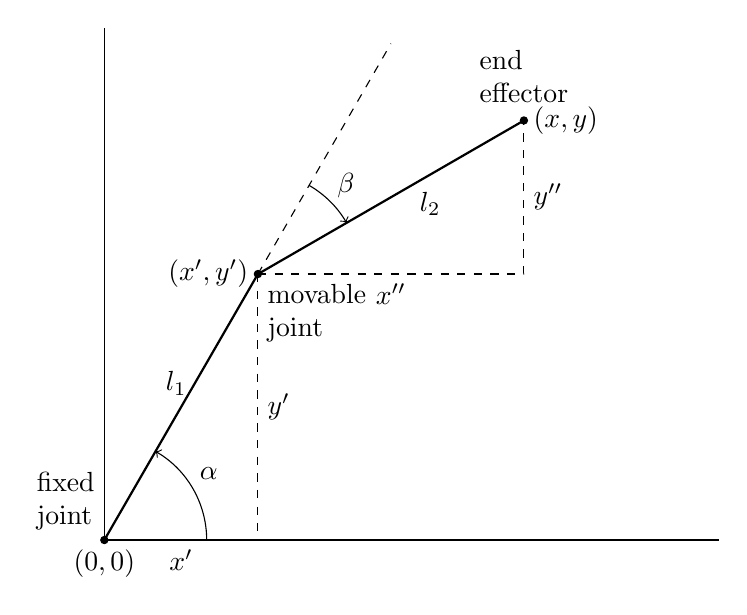
\begin{tikzpicture}[scale=1.3,align=left]
\draw (0,0) coordinate (origin) -- (6,0);
\draw (origin) -- (0,5);
\draw[thick] (origin) -- node[left,xshift=2mm,yshift=3mm] {$l_1$} ++(60:3) coordinate (prime) -- node[below,xshift=5mm,yshift=2mm] {$l_2$} ++(30:3) coordinate (point);
\path (origin) -- ++(60:3) -- ++(30:1) coordinate (angle);
\draw[dashed] (60:3) -- ++(60:2.6);
\draw[->] (1,0) arc (0:60:1) node[midway,xshift=2mm,yshift=2mm] {$\alpha$};
\draw[<-] (angle) arc (30:60:1) node[midway,xshift=2mm,yshift=2mm] {$\beta$};
\draw[fill] (origin) circle [radius=1pt] node[below] {$(0,0)$};
\draw[fill] (prime) circle [radius=1pt] node[left] {$(x',y')$};
\draw[fill] (point) circle [radius=1pt] node[right] {$(x,y)$};
\node[above,yshift=1mm] at (point) {\p{end}\\\p{effector}};
\node[above left] at (origin) {\p{fixed}\\\p{joint}};
\node[below right] at (prime) {\p{movable}\\\p{joint}};
\draw[dashed] (prime) |- (origin);
\draw[dashed] (prime) -| (point);
\path (origin) -- node[below] {$x'$} (prime |- origin);
\path (prime |- origin) -- node[right] {$y'$} (prime);
\path (prime) -- node[below] {$x''$} (prime -| point);
\path (prime -| point) -- node[right] {$y''$} (point);
\end{tikzpicture}
\end{center}
\caption{Cinemática frontal de um braço de dois elos}\label{fig.forward-kinematics}
\end{figure}

Projeto $(x',y')$ sobre os eixos $x$- e $y$-eixos; por trigonometria suas coordenadas são:
\begin{eqnarray*}
x' &=& l_1 \cos \alpha\\
y' &=& l_1 \sin \alpha\,.
\end{eqnarray*}
Agora tome $(x'',y'')$ como origem de um novo sistema de coordenadas e projete $(x,y)$ em seus eixos para obter $(x'',y'')$. A posição do efeito final ou \emph{relativa} ao novo sistema de coordenadas é:
\begin{eqnarray*}
x'' &=& l_2 \cos (\alpha+\beta)\\
y'' &=& l_2 \sin (\alpha+\beta)\,.
\end{eqnarray*}
Na Fig.~\ref{fig.forward-kinematics}, $\beta$ é negativo (uma rotação no sentido horário) então $\alpha+\beta$ é o ângulo entre o segundo elo e a linha paralela ao eixo $x$.

Combinando os resultados dá:
\begin{eqnarray*}
x &=& l_1 \cos \alpha + l_2 \cos(\alpha + \beta)\\
y &=& l_1 \sin \alpha + l_2 \sin(\alpha + \beta)\,.
\end{eqnarray*}

\noindent\textbf{Exampule} Let $l_1 = l_2 = 1$, $\alpha = 60^{\circ}$, $\beta = -30^{\circ}$. Depois:
\begin{eqnarray*}
x &=& 1\cdot\cos 60 + 1\cdot\cos(60-30) = \frac{1}{2} + \frac{\sqrt{3}}{2} = \frac{1+\sqrt{3}}{2}\\
y &=& 1\cdot\sin 60 + 1\cdot\sin(60-30) = \frac{\sqrt{3}}{2} + \frac{1}{2} = \frac{1+\sqrt{3}}{2}\,.
\end{eqnarray*}

Vamos verificar se este resultado faz sentido. A figura~\ref{fig.kinematics-triangle} mostra um triângulo formado pela adição de uma linha entre $(0,0)$ e $(x,y)$. O complemento do ângulo $\beta$ é $180-30=150$ e o triângulo é isoceles já que ambos os lados são $1$, portanto os outros ângulos do triângulo são iguais e seus valores são $(180-150)/2=15$. O ângulo que a nova linha forma com o eixo $x$ é $60-15=45$, o que é consistente com $x=y$.

\begin{figure}
\begin{center}
% Angles of the triangle
\begin{tikzpicture}[scale=1.3]
\draw (0,0) coordinate (origin) node[left] {$(0,0)$} -- (6,0);
\draw (origin) -- ++(60:3) coordinate (prime) -- ++(30:3) coordinate (point);
\path (origin) -- ++(60:3) -- ++(30:1) coordinate (angle);
\draw (origin) -- (point) node[right] {$(x,y)$};
\draw[dashed] (60:3) -- ++(60:2.6);
\draw[fill] (origin) circle [radius=1pt];
\draw[fill] (prime) circle [radius=1pt];
\draw[fill] (point) circle [radius=1pt];
\node[above,xshift=12mm,yshift=8mm] at (prime) {$\beta=30^{\circ}$};
\node[below,xshift=3mm,yshift=0mm] at (prime) {$150^{\circ}$};
\draw[->] (13mm,9mm) -- node[right,xshift=3mm] {$15^{\circ}$} (6mm,9mm);
\draw[->] (41mm,36mm) -- node[right,xshift=3mm] {$15^{\circ}$} (34mm,36mm);
\node[above right,xshift=5mm,yshift=1mm] at (origin) {$\alpha-15^{\circ}=60^{\circ}-15^{\circ}=45^{\circ}$};
\end{tikzpicture}
\end{center}
\caption{Cálculo dos ângulos}\label{fig.kinematics-triangle}
\end{figure}

\begin{framed}
\act{Cinemática frontal}{forward-kinematics}
\begin{itemize}
\item Programe seu robô para que ele trace o caminho do braço na Fig.~ref{fig.forward-kinematics}: vire à esquerda $60^{\circ}$, avance uma unidade ($1$m ou alguma outra distância conveniente), vire à direita $30^{\circ}$, avance uma unidade.
\item Medir os $x$- e $y$-distâncias do robô desde a origem e compará-las com os valores computados pelas equações da cinemática de avanço.
\end{itemize}
\end{framed}

\section{Cinemática inversa}\label{s.inverse-kinematics}

O anel cinza na Fig.~\ref{fig.workspace} mostra o {espacial de trabalho} do braço de dois elos, o conjunto de posições que o efetor final pode alcançar. (Assumimos que $l_2<l_1$.) O espaço de trabalho é circularmente simétrico, pois assumimos que não há limitações de rotação das articulações em um círculo completo entre $-180^{\circ}$ e $180^{\circ}$. Qualquer ponto como $a$ na circunferência do círculo externo é a posição mais distante do braço desde a origem; é obtido quando os dois elos estão alinhados de modo que o comprimento do braço seja $l_1+l_2$. As posições mais próximas da origem no espaço de trabalho são pontos como $b$ na circunferência do círculo interno; são obtidas quando o segundo elo é dobrado de volta no primeiro elo dando um comprimento de $l_1-l_2$. Outra posição alcançável $c$ é mostrada; há configurações \emph{two} (rotações das juntas) que fazem com que o braço seja posicionado a $c$.

\begin{figure}
\begin{center}
% Workspace of two-level arm
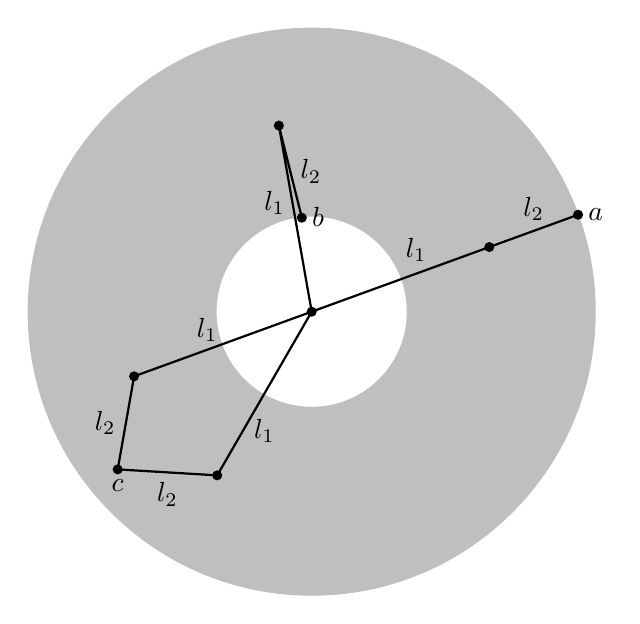
\begin{tikzpicture}[scale=.8]
% Circles
\draw[fill,gray!50] (0,0) coordinate (origin) circle[radius=45mm];
\draw[fill,white] (origin) circle[radius=15mm];
\draw[fill] (origin) circle [radius=2pt];
% First position
\draw[thick] (origin) -- node[above,xshift=2mm,yshift=1mm] {$l_1$} ++(20:30mm) -- node[above] {$l_2$} ++(20:15mm)  node[right] {$a$};
\draw[fill] (20:30mm) circle [radius=2pt];
\draw[fill] (20:45mm) circle [radius=2pt];
% Second position
\draw[thick] (origin) -- node[left,xshift=0mm,yshift=2mm] {$l_1$} ++(100:30mm) -- node[right] {$l_2$} ++(284:15mm)  node[right] {$b$};
\draw[fill] (100:30mm) circle [radius=2pt];
\draw[fill] (96:15mm) circle [radius=2pt];
% Third position
\draw[thick] (origin) -- node[above,xshift=-2mm,yshift=-1mm] {$l_1$} ++(200:30mm) coordinate (mid1) -- node[left] {$l_2$} ++(260:15mm) coordinate (endtwo) node[below] {$c$};
\draw[thick] (origin) -- node[below,,xshift=0mm,yshift=-2mm] {$l_1$} ++(240:30mm) coordinate (mid2) -- node[below] {$l_2$} (endtwo);
\draw[fill] (mid1) circle [radius=2pt];
\draw[fill] (mid2) circle [radius=2pt];
\draw[fill] (endtwo) circle [radius=2pt];
\end{tikzpicture}
\end{center}
\caption{Espaço de trabalho de um braço de duas alavancas}\label{fig.workspace}
\end{figure}

Sob a suposição de que $l_2<l_1$, nenhuma seqüência de rotações pode posicionar a extremidade do braço mais perto da origem que $l_1-l_2$ e nenhuma posição a uma distância maior que $l_1+l_2$ da origem é acessível. Pela figura aprendemos que um problema na cinemática inversa - encontrar comandos para alcançar um ponto específico - pode ter zero, uma ou muitas soluções.

O cálculo da cinemática inversa utiliza a \emph{law of cosines}. (Fig.~\ref{fig.cosines}):
\[
a^2 + b^2 - 2ab \cos \theta = c^2\,.
\]
Num triângulo à direita $\cos 90^{\circ} = 0$ e a lei reduz ao teorema de Pitágoras.

\begin{figure}
\begin{center}
% Law of cosines
\begin{tikzpicture}
\draw (0,0) coordinate (origin) --  node[below] {$c$} (6,0) coordinate (two);
\draw (origin) -- node[left] {$a$} ++(60:3) coordinate (one) -- node[above] {$b$} (two);
\node[below,xshift=1mm,yshift=-2mm] at (one) {$\theta$};
\end{tikzpicture}
\end{center}
\caption{Lei de cosseno}\label{fig.cosines}
\end{figure}

Suponha agora que nos é dado um ponto $(x,y)$ e queremos valores para $\alpha,\beta$ (se houver algum) que trará o braço a esse ponto. Figura~\ref{fig.inverse-kinematics} semelhante à Figura~\ref{fig.kinematics-triangle} exceto que os valores específicos são substituídos por ângulos e comprimentos arbitrários.

Pelo teorema de Pitágoras, $r=\sqrt{x^2 + y^2}$.

\begin{figure}
\begin{center}
% Inverse kinematics
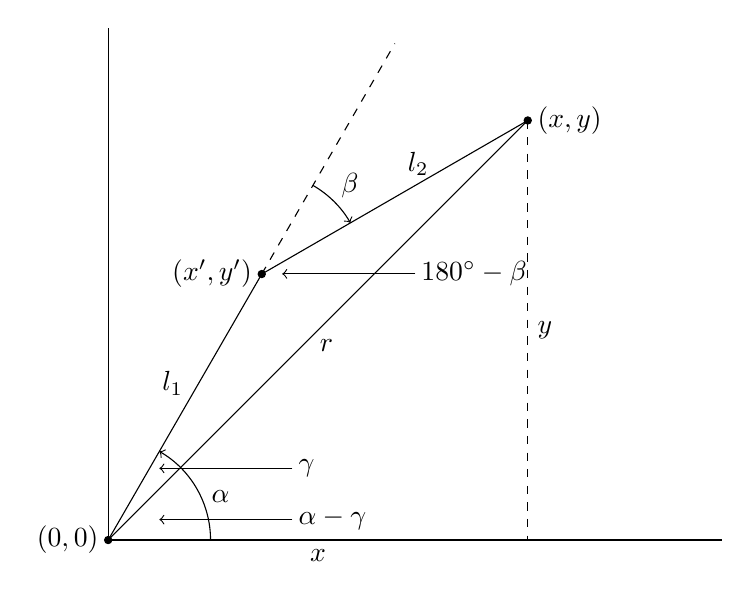
\begin{tikzpicture}[scale=1.3]
\draw (0,0) coordinate (origin) -- (6,0);
\draw (origin) -- (0,5);
\draw (origin) -- node[left,xshift=1mm,yshift=3mm] {$l_1$} ++(60:3) coordinate (prime) -- node[below,xshift=3mm,yshift=7mm] {$l_2$} ++(30:3) coordinate (point);
\draw[dashed] (point) -- node[right] {$y$} (point |- origin);
\draw (origin) -- node[below] {$x$} (origin -| point);
\path (origin) -- ++(60:3) -- ++(30:1) coordinate (angle);
\draw[dashed] (60:3) -- ++(60:2.6);
\draw (origin) -- node[right,xshift=-1mm,yshift=-2mm] {$r$} (point);
\draw[->] (1,0) arc (0:60:1) node[midway,xshift=3mm,yshift=-1mm] {$\alpha$};
\draw[<-] (angle) arc (30:60:1) node[midway,xshift=2mm,yshift=2mm] {$\beta$};
\draw[fill] (origin) circle [radius=1pt] node[left] {$(0,0)$};
\draw[fill] (prime) circle [radius=1pt] node[left] {$(x',y')$};
\draw[fill] (point) circle [radius=1pt] node[right] {$(x,y)$};

\draw[->] (30mm,26mm) -- node[right,xshift=8mm] {$180^{\circ}-\beta$} (17mm,26mm);
\draw[->] (18mm,7mm) -- node[right,xshift=8mm] {$\gamma$} (5mm,7mm);
\draw[->] (18mm,2mm) -- node[right,xshift=8mm] {$\alpha-\gamma$} (5mm,2mm);
\end{tikzpicture}
\end{center}
\caption{Cinemática inversa de um braço de dois elos}\label{fig.inverse-kinematics}
\end{figure}

A lei de cosseno dá:
\[
l_1^2 + l_2^2 - 2l_1 l_2 \cos(180^\circ-\beta) = r^2\,,
\]
que pode ser resolvido por $\beta$:
\begin{eqnarray*}
\cos(180^\circ-\beta) &=& \frac{l_1^2 + l_2^2 - r^2}{2l_1 l_2}\\
\beta &=& 180^\circ-\cos^{-1}\left(\frac{l_1^2 + l_2^2 - r^2}{2l_1 l_2}\right)\,.
\end{eqnarray*}
Para obter $\gamma$ e depois $\alpha$, use a lei de cosines com $\gamma$ como o ângulo central:
\[
\cos\gamma = \frac{l_1^2 +r^2 - l_2^2}{2l_1 r}\,.
\]
Do triângulo direito formado por $(x,y)$ que temos:
\begin{eqnarray*}
\tan(\alpha - \gamma) &=& \frac{y}{x}\\
\alpha &=& \tan^{-1} \frac{y}{x} + \gamma\,,
\end{eqnarray*}
portanto:
\[
\alpha = \tan^{-1} \frac{y}{x} + \cos^{-1}\left(\frac{l_1^2 +r^2 - l_2^2}{2l_1 r}\right)\,.
\]

\noindent\textbf{Exemplo} Suponha novamente que $l_1 = l_2 = 1$ e que o efetor final está no ponto computado a partir da cinemática de avanço:
\[
(x,y) = \left(\frac{1+\sqrt{3}}{2},\frac{1+\sqrt{3}}{2}\right)\,.
\]
Primeiro, computar $r^2$:
\[
r^2 = x^2+y^2 = \left( \frac{1+\sqrt{3}}{2}\right)^2 + \left( \frac{1+\sqrt{3}}{2}\right)^2 = 2+\sqrt{3}\,,
\]
e usá-lo no cálculo de $\beta$:
\begin{eqnarray*}
\beta &=& 180^{\circ} - \cos^{-1} \left(\frac{1^2 + 1^2 - (2+\sqrt{3})}{2\cdot 1\cdot 1}\right)\\
&=& 180^{\circ} - \cos^{-1}\left(-\frac{\sqrt{3}}{2}\right)\\
&=& 180^{\circ} \pm 150^{\circ}\\
&=& \pm 30^{\circ}\,,
\end{eqnarray*}
desde $330^{\circ}=-30^{\circ} \!\!\!\pmod{360^\circ}$. Há duas soluções porque há duas maneiras de mover o braço para $(x,y)$.

Próximo computar $\gamma$:
\begin{equation}
\gamma = \cos^{-1}\left(\frac{1^2 + r^2 - 1^2}{2\cdot 1 \cdot r}\right) = \cos^{-1}\left(\frac{r}{2}\right)= \cos^{-1}\left(\frac{\sqrt{2+\sqrt{3}}}{2}\right) = \pm 15^{\circ}\,.\label{eq.cos15}
\end{equation}
O cosseno inverso pode ser obtido numericamente em uma calculadora ou algébricamente como mostrado no Apêndice~\ref{a.cosine}.

Desde $x=y$, o cálculo de $\alpha$ é fácil:
\[
\alpha = \tan^{-1}\frac{y}{x} + \gamma = 
\tan^{-1}1 + \gamma = 45^{\circ} \pm 15^{\circ} = 
60^{\circ} \;\textrm{ou}\; 30^{\circ}\,.
\]
A solução $\alpha=60^{\circ},\beta=-30^{\circ}$ corresponde à rotação das articulações na Fig.~\ref{fig.forward-kinematics}, enquanto a solução $\alpha=30^{\circ},\beta=30^{\circ}$ corresponde à rotação das duas articulações no sentido anti-horário.

Neste caso simples, é possível resolver a equação da cinemática direta para obter fórmulas para a cinemática inversa. Em geral, isto não é possível, portanto, são utilizadas soluções numéricas aproximadas.

\begin{framed}
\act{Cinemática inversa}{inverse-kinematics}
\begin{itemize}
\item Use as fórmulas para a cinemática inversa para programar seu robô para se mover para uma coordenada especificada.
\item Meça as distâncias de $x$- e $y$-distâncias do robô desde a origem e compare-as com as coordenadas especificadas.
\item Se o computador de seu robô não tiver a capacidade de computar as fórmulas, computá-las off-line e depois inserir os comandos no robô.
\end{itemize}
\end{framed}

%%%%%%%%%%%%%%%%%%%%%%%%%%%%%%%%%%%%%%%%%%%%%%%%%%%%%%%%%%%

\section{Rotações}\label{s.rotations}

O movimento de um manipulador robótico é descrito em termos de \emph{coordenate frames}. Três armações estão associadas ao braço na Fig.~\ref{fig.forward-kinematics}: uma armação está associada à articulação na origem (que supomos estar fixada a uma mesa ou ao chão), uma segunda armação está associada à articulação entre as duas ligações, e uma terceira armação está associada ao efetor final no final da segunda ligação.

Nesta seção descrevemos como o movimento de rotação de um braço robótico pode ser modelado matematicamente usando \emph{rotation matrizes de rotação}. Os links nos braços robóticos introduzem \emph{translations}: a segunda junta é compensada por uma distância linear de $l_1$ da primeira junta, e o efetor final é compensado por uma distância linear de $l_2$ da segunda junta. O tratamento matemático das traduções utiliza uma extensão de matrizes de rotação chamada \emph{homogeneous transforms}.

As rotações podem ser confusas porque uma matriz de rotação pode ter três interpretações que são descritas nas seguintes subseções: rotação de um vetor, rotação de um quadro de coordenadas e transformação de um vetor de um quadro de coordenadas para outro.

\subsection{Girando um vetor}

Considere um vetor com coordenadas cartesianas $(x,y)$ e coordenadas polares $(r,\phi)$ (Fig.~\ref{fig.one-vector}). Agora, gire o vetor por um ângulo $(x,y)$ e coordenadas polares $(r,y)$ (Fig.~\ref{fig.rotated-vector}). Suas coordenadas polares são $(r,\phi+theta)$. Quais são suas coordenadas cartesianas?
\begin{figure}
\begin{minipage}{.48\textwidth}
\begin{tikzpicture}[scale=1.2]
\draw (0,0) coordinate (origin) -- (4,0);
\draw (origin) -- (0,3);
\path[->] (origin) -- ++(30:3.5) coordinate (point);
\draw[->] (origin) -- node[above] {$r$} ++(30:3.46);
\draw[fill] (point) circle [radius=1pt];
\draw (point) -- node[right] {$y$} (point |- origin);
\draw (origin) -- node[below,xshift=2mm] {$x$} (point |- origin);
\draw (1,0) arc (0:30:1) node[midway,xshift=3mm] {$\phi$};
\draw[fill] (origin) circle [radius=1pt];
\end{tikzpicture}
\caption{Um vetor}\label{fig.one-vector}
\end{minipage}
\hspace{\fill}
\begin{minipage}{.48\textwidth}
\begin{tikzpicture}[scale=1.2]
\draw (0,0) coordinate (origin) -- (4,0);
\draw (origin) -- (0,3);
\path[->] (origin) -- ++(60:3.5) coordinate (point);
\draw[->] (origin) -- node[above] {$r$} ++(60:3.46);
\draw[fill] (point) circle [radius=1pt];
\draw (point) -- node[right] {$y'$} (point |- origin);
\draw (origin) -- node[below,xshift=2mm] {$x'$} (point |- origin);
\draw (1,0) arc (0:60:1);
\node at (1.2,.7) {$\phi+\theta$};
\draw[fill] (origin) circle [radius=1pt];
\end{tikzpicture}
\caption{O vetor girado por $\theta$}\label{fig.rotated-vector}
\end{minipage}
\end{figure}

%\begin{figure}
%\subfigures
%\begin{minipage}{\textwidth}
%\leftfigure{
%\begin{tikzpicture}[scale=1.3]
%\draw (0,0) coordinate (origin) -- (4,0);
%\draw (origin) -- (0,3);
%\path[->] (origin) -- ++(30:3.5) coordinate (point);
%\draw[->] (origin) -- node[above] {$r$} ++(30:3.46);
%\draw[fill] (point) circle [radius=1pt];
%\draw (point) -- node[right] {$y$} (point |- origin);
%\draw (origin) -- node[below,xshift=2mm] {$x$} (point |- origin);
%\draw (1,0) arc (0:30:1) node[midway,xshift=3mm] {$\phi$};
%\draw[fill] (origin) circle [radius=1pt];
%\end{tikzpicture}
%}
%\hspace{\fill}
%\rightfigure{
%\begin{tikzpicture}[scale=1.3]
%\draw (0,0) coordinate (origin) -- (4,0);
%\draw (origin) -- (0,3);
%\path[->] (origin) -- ++(60:3.5) coordinate (point);
%\draw[->] (origin) -- node[above] {$r$} ++(60:3.46);
%\draw[fill] (point) circle [radius=1pt];
%\draw (point) -- node[right] {$y'$} (point |- origin);
%\draw (origin) -- node[below,xshift=2mm] {$x'$} (point |- origin);
%\draw (1,0) arc (0:60:1);
%\node at (1.2,.7) {$\phi+\theta$};
%\draw[fill] (origin) circle [radius=1pt];
%\end{tikzpicture}
%}
%\leftcaption{A vector}\label{fig.one-vector}
%\rightcaption{The vector rotated by $\theta$}\label{fig.rotated-vector}
%\end{minipage}
%\end{figure}

Usando as identidades trigonométricas para a soma de dois ângulos e a conversão de $(r,\phi)$ para $(x,y)$ que temos:
\begin{eqnarray*}
x' &=& r\cos(\phi+\theta)\\
&=&r\cos\phi\cos\theta - r\sin\phi\sin\theta\\
&=&(r\cos\phi)\cos\theta - (r\sin\phi)\sin\theta\\
&=&x\cos\theta - y\sin\theta\,,\\
\\
y' &=& r\sin(\phi+\theta)\\
&=&r\sin\phi\cos\theta + r\cos\phi\sin\theta\\
&=&(r\sin\phi)\cos\theta + (r\cos\phi)\sin\theta\\
&=&y\cos\theta + x\sin\theta\\
&=&x\sin\theta + y\cos\theta\,.\\
\end{eqnarray*}
Estas equações podem ser expressas como a multiplicação de uma matriz chamada \emph{rotation matrix} e um vetor:
\[
\spacearray
\left[\begin{array}{c}x'\\y'\end{array}\right]=
\left[\begin{array}{cc}\cos\theta&-\sin\theta\\\sin\theta&\cos\theta\end{array}\right]
\left[\begin{array}{c}x\\y\end{array}\right]\,.
\]
\noindent\textbf{Exemplo} Que $p$ seja o ponto na ponta de um vetor de comprimento $r=1$ que forma um ângulo de $\phi=30^{\circ}$ com o positivo $x$-eixo. As coordenadas cartesianas de $p$ são $\left(\frac{\sqrt{3}}{2},\,\frac{1}{2}\right)$. Suponha que o vetor seja girado por $\theta=30^{\circ}$. Quais são as novas coordenadas cartesianas de $p$? Usando a multiplicação matricial:
\[
\spacearray
\left[\begin{array}{c}x'\\y'\end{array}\right]\;=\;
\left[\begin{array}{cc}\frac{\sqrt{3}}{2}&-\frac{1}{2}\\\frac{1}{2}&\frac{\sqrt{3}}{2}\end{array}\right]
\left[\begin{array}{c}\frac{\sqrt{3}}{2}\\\frac{1}{2}\end{array}\right]\;=\;
\left[\begin{array}{c}\frac{1}{2}\\\frac{\sqrt{3}}{2}\end{array}\right]\,.
\]
O resultado faz sentido porque girar um vetor cujo ângulo com o eixo $x$ é $30^{\circ}$ por $30^{\circ}$ deve dar um vetor cujo ângulo com o eixo $x$ é $60^{\circ}$.

Suponha que o vetor seja girado por um adicional de $30^{\circ}$; suas novas coordenadas são:
\begin{equation}\label{eq.rotate1}
\spacearray
\left[\begin{array}{cc}\frac{\sqrt{3}}{2}&-\frac{1}{2}\\\frac{1}{2}&\frac{\sqrt{3}}{2}\end{array}\right]\;\;
\left(\left[\begin{array}{cc}\frac{\sqrt{3}}{2}&-\frac{1}{2}\\\frac{1}{2}&\frac{\sqrt{3}}{2}\end{array}\right]
\left[\begin{array}{c}\frac{\sqrt{3}}{2}\\\frac{1}{2}\end{array}\right]\right)\;=\;
\left[\begin{array}{cc}\frac{\sqrt{3}}{2}&-\frac{1}{2}\\\frac{1}{2}&\frac{\sqrt{3}}{2}\end{array}\right]
\left[\begin{array}{c}\frac{1}{2}\\\frac{\sqrt{3}}{2}\end{array}\right]\;=\;
\left[\begin{array}{c}0\\1\end{array}\right]\,.
\end{equation}
Este resultado também faz sentido. A rotação de um vetor cujo ângulo é de $30^{\circ}$ duas vezes por $30^{\circ}$ (para um total de $60^{\circ}$) deve dar $90^{\circ}$. O co-seno de $90^{\circ}$ é $0$ e o seno de $90^{\circ}$ é $1$.

Como a multiplicação matricial é associativa, a multiplicação também poderia ser feita da seguinte forma:
\begin{equation}\label{eq.rotate2}
\spacearray
\left(\left[\begin{array}{cc}\frac{\sqrt{3}}{2}&-\frac{1}{2}\\\frac{1}{2}&\frac{\sqrt{3}}{2}\end{array}\right]
\left[\begin{array}{cc}\frac{\sqrt{3}}{2}&-\frac{1}{2}\\\frac{1}{2}&\frac{\sqrt{3}}{2}\end{array}\right]\right)\;\;
\left[\begin{array}{c}\frac{\sqrt{3}}{2}\\\frac{1}{2}\end{array}\right]\,.
\end{equation}

\begin{framed}
\act{Matrizes de rotação}{rotation-matrix}
\begin{itemize}
\item Demonstrar a associatividade da multiplicação da matriz mostrando que a multiplicação em Eq.~ref{eq.rotate2} dá o mesmo resultado que a multiplicação em Eq.~\ref{eq.rotate1}.
\item Calcular a matriz para uma rotação de $-30^{\circ}$ e mostrar que a multiplicação desta matriz pela matriz para uma rotação de $30^{\circ}$ dá a matriz para uma rotação de $0^{\circ}$.
\item Este item é uma multiplicação comutativa?
\item A multiplicação de matrizes de rotação bidimensionais é comutativa?
\end{itemize}
\end{framed}

\subsection{Girando uma estrutura de coordenadas}

Vamos reinterpretar Figs.~\ref{fig.one-vector}--\ref{fig.rotated-vector}. A figura~\ref{fig.one-frame} mostra um quadro de coordenadas (azul) definido por dois vetores de unidade ortogonais:
\[
\vec{x}= \left[\begin{array}{c}1\\0\end{array}\right]\,,\;\;
\vec{y}= \left[\begin{array}{c}0\\1\end{array}\right]\,.
\]
Fig.~\ref{fig.frame-rotated} mostra o \emph{coordenate frame} girado em $\theta$ graus (vermelho). Os novos vetores de unidade $\vec{x'}$ e $\vec{y'}$ podem ser obtidos pela multiplicação pela matriz de rotação derivada acima:
\begin{eqnarray*}
\vec{x'}&=&
\left[\spacearray\begin{array}{cc}\cos\theta&-\sin\theta\\\sin\theta&\cos\theta\end{array}\right]
\left[\spacearray\begin{array}{c}1\\0\end{array}\right]=
\left[\spacearray\begin{array}{l}\cos \theta\\\sin\theta\;\;\:\end{array}\right]\\
\,\\
\vec{y'}&=&
\left[\spacearray\begin{array}{cc}\cos\theta&-\sin\theta\\\sin\theta&\cos\theta\end{array}\right]
\left[\spacearray\begin{array}{c}0\\1\end{array}\right]=
\left[\spacearray\begin{array}{l}-\sin \theta\\\cos\theta\end{array}\right]\,.
\end{eqnarray*}
\begin{figure}
\begin{minipage}{.48\textwidth}
\begin{tikzpicture}[scale=1.2]
\draw (0,0) coordinate (origin) -- (3.4,0);
\draw (origin) -- (0,2.8);
\draw[->,thick,blue] (0,0) -- node[below] {$\vec{x}$} (2,0);
\draw[->,thick,blue] (0,0) -- node[left] {$\vec{y}$} (0,2);
\end{tikzpicture}
\caption{Moldura de coordenadas original (azul)}\label{fig.one-frame}
\end{minipage}
\hspace{\fill}
\begin{minipage}{.48\textwidth}
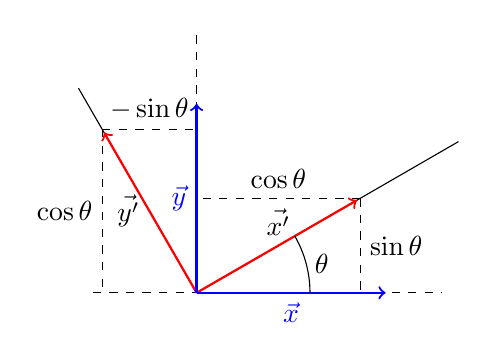
\begin{tikzpicture}[scale=1.2]
\begin{scope}[rotate=30]
\draw (0,0) coordinate (origin) -- (3.2,0);
\draw (origin) -- (0,2.5);
\path (0,0) -- node[above] {$\vec{x'}$} (2,0) coordinate (xprime);
\path (0,0) -- node[left] {$\vec{y'}$} (0,2) coordinate (yprime);
\draw[->,thick,red] (0,0) -- (1.96,0);
\draw[->,thick,red] (0,0) -- (0,1.96);
\end{scope}
\draw[dashed] (-1.1,0) -- (origin) -- (2.6,0);
\draw[dashed] (origin) -- (0,2.8);
\draw[->,thick,blue] (0,0) -- node[below] {$\vec{x}$} (2,0);
\draw[->,thick,blue] (0,0) -- node[left] {$\vec{y}$} (0,2);
\draw[dashed] (xprime) -- node[right] {$\sin \theta$} (xprime |- origin);
\draw[dashed] (xprime) -- node[above] {$\cos \theta$} (origin |- xprime);
\draw[dashed] (yprime) -- node[left] {$\cos \theta$} (yprime |- origin);
\draw[dashed] (yprime) -- node[above] {$-\sin \theta$} (origin |- yprime);
\draw (1.2,0) arc (0:30:1.2) node[midway,xshift=2mm,yshift=0mm] {$\theta$};
\end{tikzpicture}
\caption{Nova moldura de coordenadas (vermelho) obtida pela rotação da moldura de coordenadas original (azul) por $\theta$}\label{fig.frame-rotated}
\end{minipage}
\end{figure}

%\begin{figure}
%\subfigures
%\begin{minipage}{\textwidth}
%\leftfigure{
%\begin{tikzpicture}[scale=1.3]
%\draw (0,0) coordinate (origin) -- (3.4,0);
%\draw (origin) -- (0,2.8);
%\draw[->,thick,blue] (0,0) -- node[below] {$\vec{x}$} (2,0);
%\draw[->,thick,blue] (0,0) -- node[left] {$\vec{y}$} (0,2);
%\end{tikzpicture}
%}
%\hspace{\fill}
%\rightfigure{
%\begin{tikzpicture}[scale=1.3]
%\begin{scope}[rotate=30]
%\draw (0,0) coordinate (origin) -- (3.2,0);
%\draw (origin) -- (0,2.5);
%\path (0,0) -- node[above] {$\vec{x'}$} (2,0) coordinate (xprime);
%\path (0,0) -- node[left] {$\vec{y'}$} (0,2) coordinate (yprime);
%\draw[->,thick,red] (0,0) -- (1.96,0);
%\draw[->,thick,red] (0,0) -- (0,1.96);
%\end{scope}
%\draw[dashed] (-1.1,0) -- (origin) -- (2.6,0);
%\draw[dashed] (origin) -- (0,2.8);
%\draw[->,thick,blue] (0,0) -- node[below] {$\vec{x}$} (2,0);
%\draw[->,thick,blue] (0,0) -- node[left] {$\vec{y}$} (0,2);
%\draw[dashed] (xprime) -- node[right] {$\sin \theta$} (xprime |- origin);
%\draw[dashed] (xprime) -- node[above] {$\cos \theta$} (origin |- xprime);
%\draw[dashed] (yprime) -- node[left] {$\cos \theta$} (yprime |- origin);
%\draw[dashed] (yprime) -- node[above] {$-\sin \theta$} (origin |- yprime);
%\draw (1.2,0) arc (0:30:1.2) node[midway,xshift=2mm,yshift=0mm] {$\theta$};
%\end{tikzpicture}
%}
%\leftcaption{Original coordinate frame (blue)}\label{fig.one-frame}
%\rightcaption{New coordinate frame (red) obtained by rotating the original coordinate frame (blue) by $\theta$}\label{fig.frame-rotated}
%\end{minipage}
%\end{figure}
\noindent\textbf{Exemplo} Para os vetores de unidade em Fig.~\ref{fig.one-frame} e uma rotação de $30^\circ$:
\begin{eqnarray*}
\vec{x'}&=&\left[\spacearray\begin{array}{cc}\frac{\sqrt{3}}{2}&-\frac{1}{2}\\\frac{1}{2}&\frac{\sqrt{3}}{2}\end{array}\right]
\left[\spacearray\begin{array}{c}1\\0\end{array}\right]=
\left[\spacearray\begin{array}{c}\frac{\sqrt{3}}{2}\\\frac{1}{2}\end{array}\right]\\
\,\\
\vec{y'}&=&\left[\spacearray\begin{array}{cc}\frac{\sqrt{3}}{2}&-\frac{1}{2}\\\frac{1}{2}&\frac{\sqrt{3}}{2}\end{array}\right]
\left[\spacearray\begin{array}{c}0\\1\end{array}\right]=
\left[\spacearray\begin{array}{c}-\frac{1}{2}\\\frac{\sqrt{3}}{2}\end{array}\right]\,.
\end{eqnarray*}

\subsection{Transformar um vetor de um quadro de coordenadas para outro}

Deixe a origem de uma armação coordenada $b$ (azul) representar a junta de um efetor final como um soldador e deixe o ponto $p$ ser a ponta do soldador (Fig.~\ref{fig.frameb}). Por convenção em robótica, o quadro de coordenadas de uma entidade é denotado por um superescrito ``pre''. Nota de rodapé (A convenção é utilizar letras maiúsculas tanto para o quadro quanto para as coordenadas, mas utilizamos letras minúsculas para maior clareza).  No quadro $b$, o ponto $\bp$ tem coordenadas polares $(r,\phi)$ e coordenadas cartesianas $(\bx,\bx,\by)$ relacionadas pelas fórmulas trigonométricas usuais:
\[
\bp = (\bx,\by) = (r\cos\phi,\, r\sin\phi)\,.
\]

\begin{figure}
\begin{minipage}{.48\textwidth}
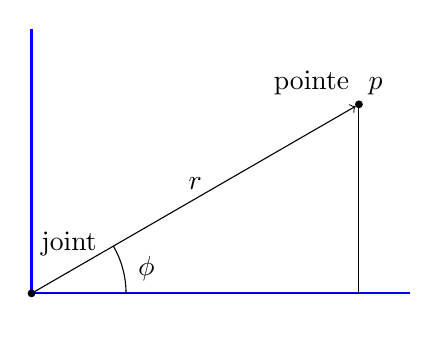
\begin{tikzpicture}[scale=1.2]
\draw[thick,blue] (0,0) coordinate (origin) -- (4,0);
\draw[thick,blue] (origin) -- (0,2.8);
\path (origin) -- node[above] {$r$} ++(30:4) coordinate (point) node[above right] {$p$};
\draw[->] (origin) -- ++(30:3.96);
\draw[fill] (point) circle [radius=1pt] node[above left] {\p{pointe}};
\draw (point) -- node[right] {$\by$} (point |- origin);
\draw (origin) -- node[below,xshift=2mm] {$\bx$} (point |- origin);
\draw (1,0) arc (0:30:1) node[midway,xshift=3mm] {$\phi$};
\draw[fill] (origin) circle [radius=1pt] node[above right,yshift=10pt] {\p{joint}};
\end{tikzpicture}
\caption{Aponte $p$ na ponta de um efetor final em moldura coordenada $b$ (azul)}\label{fig.frameb}
\end{minipage}
\hspace{\fill}
\begin{minipage}{.48\textwidth}
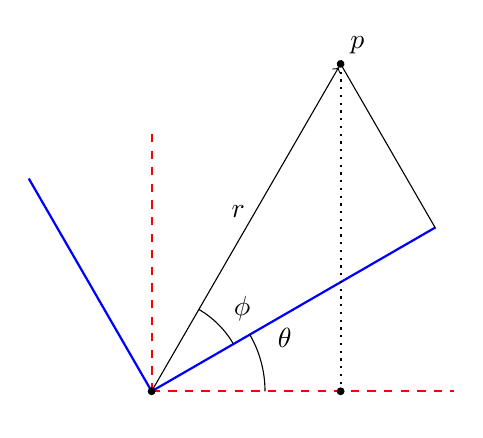
\begin{tikzpicture}[scale=1.2]
\begin{scope}[rotate=30]
\draw[thick,blue] (0,0) coordinate (origin) -- node[black,below,xshift=12mm,yshift=6mm] {$\bx$} (3.47,0);
\draw[thick,blue] (origin) -- (0,2.6);
\path (origin) -- node[above,xshift=-1mm] {$r$} ++(30:4) coordinate (point) node[above right] {$p$};
\draw[->] (origin) -- ++(30:3.96);
\draw[fill] (point) circle [radius=1pt];
\draw (point) -- node[right] {$\by$} (point |- origin);
\draw (1,0) arc (0:30:1) node[midway,xshift=3mm,yshift=2mm] {$\phi$};
\end{scope}
\draw[thick,dashed,red] (origin) -- (3.2,0);
\draw[thick,dashed,red] (origin) -- (0,2.8);
\draw[thick,dotted] (point) -- node[right] {$\ay$} (point |- origin);
\draw[fill] (point |- origin) circle [radius=1pt];
\path[dashed] (origin) -- node[below,xshift=2mm] {$\ax$} (point |- origin);
\draw (1.2,0) arc (0:30:1.2) node[midway,xshift=3mm,yshift=3mm] {$\theta$};
\draw[fill] (origin) circle [radius=1pt];
\end{tikzpicture}
\caption{Ponto $p$ em armações coordenadas $a$ (vermelho) e $b$ (azul)}\label{fig.framea}
\end{minipage}
\end{figure}

%\begin{figure}
%\subfigures
%\begin{minipage}{\textwidth}
%\leftfigure{
%\begin{tikzpicture}[scale=1.3]
%\draw[thick,blue] (0,0) coordinate (origin) -- (4,0);
%\draw[thick,blue] (origin) -- (0,2.8);
%\path (origin) -- node[above] {$r$} ++(30:4) coordinate (point) node[above right] {$p$};
%\draw[->] (origin) -- ++(30:3.96);
%\draw[fill] (point) circle [radius=1pt] node[above left] {\p{tip}};
%\draw (point) -- node[right] {$\by$} (point |- origin);
%\draw (origin) -- node[below,xshift=2mm] {$\bx$} (point |- origin);
%\draw (1,0) arc (0:30:1) node[midway,xshift=3mm] {$\phi$};
%\draw[fill] (origin) circle [radius=1pt] node[above right,yshift=10pt] {\p{joint}};
%\end{tikzpicture}
%}
%\hspace{\fill}
%\rightfigure{
%\begin{tikzpicture}[scale=1.3]
%\begin{scope}[rotate=30]
%\draw[thick,blue] (0,0) coordinate (origin) -- node[black,below,xshift=12mm,yshift=6mm] {$\bx$} (3.47,0);
%\draw[thick,blue] (origin) -- (0,2.6);
%\path (origin) -- node[above,xshift=-1mm] {$r$} ++(30:4) coordinate (point) node[above right] {$p$};
%\draw[->] (origin) -- ++(30:3.96);
%\draw[fill] (point) circle [radius=1pt];
%\draw (point) -- node[right] {$\by$} (point |- origin);
%\draw (1,0) arc (0:30:1) node[midway,xshift=3mm,yshift=2mm] {$\phi$};
%\end{scope}
%\draw[thick,dashed,red] (origin) -- (3.2,0);
%\draw[thick,dashed,red] (origin) -- (0,2.8);
%\draw[thick,dotted] (point) -- node[right] {$\ay$} (point |- origin);
%\draw[fill] (point |- origin) circle [radius=1pt];
%\path[dashed] (origin) -- node[below,xshift=2mm] {$\ax$} (point |- origin);
%\draw (1.2,0) arc (0:30:1.2) node[midway,xshift=3mm,yshift=3mm] {$\theta$};
%\draw[fill] (origin) circle [radius=1pt];
%\end{tikzpicture}
%}
%\leftcaption{Point $p$ at the tip of an end effector in coordinate frame $b$ (blue)}\label{fig.frameb}
%\rightcaption{Point $p$ in coordinate frames $a$ (red) and $b$ (blue)}\label{fig.framea}
%\end{minipage}
%\end{figure}

Suponha que a junta (\emph{com sua estrutura de coordenadas}) seja girada pelo ângulo de $\theta$. As coordenadas do ponto em relação a $b$ permanecem as mesmas, mas a estrutura de coordenadas se moveu, então perguntamos: Quais são as coordenadas $ap=(\ax,\ay)$ do ponto na estrutura de coordenadas antes de ser movida? Na Fig.~\ref{fig.framea} a moldura original $b$ é mostrada girada para uma nova posição (e ainda é mostrada em azul), enquanto a moldura de coordenadas $a$ está na posição antiga de $b$ e é mostrada como linhas tracejadas vermelhas. Na seção anterior, perguntamos como transformar uma moldura de coordenadas em outra; aqui, perguntamos como transformar as coordenadas de um ponto em uma moldura em suas coordenadas em outra moldura.

Em termos do braço robótico: nós sabemos $(\bx,\by)$, as coordenadas da ponta do efetor final em relação ao quadro do efetor final, e agora pedimos suas coordenadas $\ap=(\ax,\ay)$ em relação à base fixa. Isto é importante porque se soubermos $\ap$, podemos calcular a distância e o ângulo desde a ponta do soldador até as partes do carro que ele deve agora soldar.

Podemos repetir o cálculo utilizado para a rotação de um vetor:
\begin{eqnarray*}
\ax &=& r\cos(\phi+\theta)\\
&=&r\cos\phi\cos\theta - r\sin\phi\sin\theta\\
&=&\bx\cos\theta - \by\sin\theta\,,\\
\\
\ay &=& r\sin(\phi+\theta)\\
&=&r\sin\phi\cos\theta + r\cos\phi\sin\theta\\
&=&\bx\sin\theta + \by\cos\theta\,,\\
\end{eqnarray*}
para obter a matriz de rotação:
\begin{equation}
\spacearray
\left[\begin{array}{c}\ax\\\ay\end{array}\right]=
\left[\begin{array}{cc}\cos\theta&-\sin\theta\\\sin\theta&\cos\theta\end{array}\right]
\left[\begin{array}{c}\bx\\\by\end{array}\right]\,.\label{eq.frame-to-frame}
\end{equation}
A matriz é chamada de matriz de rotação $b$ emoldurada para $a$ emoldurada e designada por $leftidx{^a_b}{R}$. A pré-multiplicação do ponto $bp$ na moldura $b$ pela matriz de rotação dá $ap$ suas coordenadas na moldura $a$:
\[
\ap = \leftidx{^a_b}{R}{} \; \bp\,.
\]
\noindent\textbf{Exemplo} Que $\bp$ seja o ponto na moldura $b$ na ponta de um vetor de comprimento $r=1$ que forma um ângulo de $\phi=30^{\circ}$ com o positivo $x$-eixo. As coordenadas de $\bp$ são $\left(\frac{\sqrt{3}}{2},\,\frac{1}{2}\right)$. Suponha que o quadro de coordenadas $b$ (juntamente com o ponto $p$) seja girado por $theta=30^{\circ}$ para obter o quadro de coordenadas $a$. Quais são as coordenadas de $ap$? Usando Eq.~ref{eq.frame-to frame}:
\[
\spacearray
\ap=
\left[\begin{array}{c}\ax\\\ay\end{array}\right]\;=\;
\left[\begin{array}{cc}\frac{\sqrt{3}}{2}&-\frac{1}{2}\\\frac{1}{2}&\frac{\sqrt{3}}{2}\end{array}\right]
\left[\begin{array}{c}\frac{\sqrt{3}}{2}\\\frac{1}{2}\end{array}\right]\;=\;
\left[\begin{array}{c}\frac{1}{2}\\\frac{\sqrt{3}}{2}\end{array}\right]\,.
\]
Se o frame $a$ for agora girado $30^{\circ}$, obtemos as coordenadas do ponto em um terceiro frame $a1$. Pré-multiplicar $ap$ pela matriz de rotação por $30^{\circ}$ para obter $\aprimep$:
\[
\spacearray
\aprimep = \left[\begin{array}{cc}\frac{\sqrt{3}}{2}&-\frac{1}{2}\\\frac{1}{2}&\frac{\sqrt{3}}{2}\end{array}\right]\;\;
\left(\left[\begin{array}{cc}\frac{\sqrt{3}}{2}&-\frac{1}{2}\\\frac{1}{2}&\frac{\sqrt{3}}{2}\end{array}\right]
\left[\begin{array}{c}\frac{\sqrt{3}}{2}\\\frac{1}{2}\end{array}\right]\right)\;=\;
\left[\begin{array}{cc}\frac{\sqrt{3}}{2}&-\frac{1}{2}\\\frac{1}{2}&\frac{\sqrt{3}}{2}\end{array}\right]
\left[\begin{array}{c}\frac{1}{2}\\\frac{\sqrt{3}}{2}\end{array}\right]\;=\;
\left[\begin{array}{c}0\\1\end{array}\right]\,.
\]
O produto das duas matrizes de rotação:
\[
\spacearray
\left[\begin{array}{cc}\frac{\sqrt{3}}{2}&-\frac{1}{2}\\\frac{1}{2}&\frac{\sqrt{3}}{2}\end{array}\right]
\left[\begin{array}{cc}\frac{\sqrt{3}}{2}&-\frac{1}{2}\\\frac{1}{2}&\frac{\sqrt{3}}{2}\end{array}\right]=
\left[\begin{array}{cc}\frac{1}{2}&-\frac{\sqrt{3}}{2}\\\frac{\sqrt{3}}{2}&\frac{1}{2}\end{array}\right]
\]
resulta na matriz de rotação para a rotação da moldura de coordenadas original $b$ por $60^{\circ}$:
\[
\spacearray
\left[\begin{array}{cc}\frac{1}{2}&-\frac{\sqrt{3}}{2}\\\frac{\sqrt{3}}{2}&\frac{1}{2}\end{array}\right]
\left[\begin{array}{c}\frac{\sqrt{3}}{2}\\\frac{1}{2}\end{array}\right]\;=\;
\left[\begin{array}{c}0\\1\end{array}\right]\,.
\]

Dada uma seqüência de rotações, a pré-multiplicação de suas matrizes de rotação dá a matriz de rotação para a rotação equivalente à soma das rotações individuais.

\section{Rotação e tradução de um quadro de coordenadas}\label{s.rotate-translate}

As juntas nos manipuladores robóticos são conectadas por links, de modo que os sistemas de coordenadas são relacionados não apenas por rotações, mas também por traduções. O ponto $p$ na Fig.~\ref{fig.before-rotate} representa um ponto no quadro de coordenadas (vermelho) $b$, mas relativo ao quadro de coordenadas (azul tracejado) $a$, o quadro $b$ é girado pelo ângulo $theta$ e sua origem é traduzida por $Delta x$ e $Delta y$. Se $\bp=(\bx,\by)$, as coordenadas do ponto na moldura $b$, são conhecidas, quais são suas coordenadas $\ap=(\ax,\ay)$ na moldura $a$?

\begin{figure}
\begin{center}
\begin{tikzpicture}[scale=1.3]
\begin{scope}[yshift=1cm,xshift=3cm,rotate around={30:(0,0)}]
\draw[thick,red] (0,0) coordinate (origin) -- node[black,near end,xshift=8mm,yshift=-2mm] {\p{frame b}} (4,0);
\draw[thick,red] (origin) -- (0,3);
\path (origin) -- node[above,xshift=-1mm] {$r$} ++(30:4) coordinate (point) node[above right] {$p$};
\draw[->] (origin) -- ++(30:3.96);
\draw[fill] (point) circle [radius=1pt];
\draw (point) -- node[right] {$\by$} (point |- origin);
\path (origin) -- node[below,xshift=5mm,yshift=2mm] {$\bx$} (point |- origin);
\draw (1,0) arc (0:30:1) node[midway,xshift=3mm,yshift=2mm] {$\phi$};
\end{scope}
\draw[dashed,thick,blue] (0,0) coordinate (origina) -- node[black,below,midway,yshift=-1mm] {\p{frame a}} (6,0);
\draw[dashed,thick,blue] (origina) -- (0,3);
\draw[->] (origina) -- ($ (origina) ! .985 ! (point) $);
\draw[dashed] (origin) -- (point |- origin);
\draw (4.5,1) arc (0:30:1.45) node[midway,xshift=2mm] {$\theta$};
\draw[dotted,thick] (origin) -- (origin |- origina) node [right,midway] {$\Delta y$};
\draw[dotted,thick] (origin) -- (origina |- origin) node [below,midway] {$\Delta x$};
\draw[fill] (origin) circle [radius=1pt];
\draw[fill] (origina) circle [radius=1pt];
\end{tikzpicture}
\caption{A moldura $b$ é girada e traduzida para moldura $a$}\label{fig.before-rotate}
\end{center}
\end{figure}

Para realizar este cálculo, definimos um quadro de coordenadas intermediário (verde) $a1$ que tem a mesma origem que $b$ e a mesma orientação que $a$ (Fig.~\ref{fig.after-rotate}). Quais são as coordenadas $\aprimep=(\aprimex,\aprimey)$ do ponto na moldura $a1$? Esta é simplesmente a rotação de $\theta$ que já fizemos antes:
\[
\spacearray
\aprimep=\left[\begin{array}{c}\aprimex\\\aprimey\end{array}\right]=
\left[\begin{array}{cc}\cos\theta&-\sin\theta\\\sin\theta&\cos\theta\end{array}\right]
\left[\begin{array}{c}\bx\\\by\end{array}\right]\,.
\]
Agora que temos as coordenadas do ponto em $a1$, é fácil obter as coordenadas no quadro $a$, acrescentando os offsets da tradução. Em forma de matriz:
\[
\spacearray
\ap=\left[\begin{array}{c}\ax\\\ay\end{array}\right]=
\left[\begin{array}{c}\aprimex\\\aprimey\end{array}\right]\,+\,
\left[\begin{array}{c}\Delta x\\\Delta y\end{array}\right]\,.
\]

\begin{figure}
\begin{center}
\begin{tikzpicture}[scale=1.3]
\begin{scope}[yshift=1cm,xshift=3cm,rotate around={30:(0,0)}]
\draw[thick,red] (0,0) coordinate (origin) -- node[black,near end,xshift=8mm,yshift=-2mm] {\p{frame b}} (4,0);
\draw[thick,red] (origin) -- (0,3);
\path (origin) -- ++(30:4) coordinate (point) node[above right] {$p$};
\draw[->] (origin) -- ++(30:3.96);
\draw[fill] (point) circle [radius=1pt];
\draw (1,0) arc (0:30:1) node[midway,xshift=3mm,yshift=2mm] {$\phi$};
\end{scope}
\draw[thick,green!60!black] (origin) -- node[black,below,midway,xshift=4mm] {\p{frame a1}} +(4,0);
\draw[thick,green!60!black] (origin) -- +(0,4);
\draw[dotted,thick] (point) -- node [right,midway] {$\aprimey$} (point |- origin);
\draw[dotted,thick] (point) -- node [above,midway] {$\aprimex$} (origin |- point);
\draw[dashed,thick,blue] (0,0) coordinate (origina) -- node[black,below,midway,yshift=-1mm] {\p{frame a}} (6,0);
\draw[dashed,thick,blue] (origina) -- (0,3);
\draw[->] (origina) -- ($ (origina) ! .985 ! (point) $);
\draw (4.5,1) arc (0:30:1.45) node[midway,xshift=2mm] {$\theta$};
\draw[dotted,thick] (origin) -- (origin |- origina) node [right,midway] {$\Delta y$};
\draw[dotted,thick] (origin) -- (origina |- origin) node [below,midway] {$\Delta x$};
\draw[fill] (origin) circle [radius=1pt];
\draw[fill] (origina) circle [radius=1pt];
\end{tikzpicture}
\caption{A moldura $b$ é girada para a moldura $a1$ e depois traduzida para a moldura $a$}\label{fig.after-rotate}
\end{center}
\end{figure}

\emph{Tratamentos homogêneos} são usados para combinar uma rotação e uma tradução em um único operador. O vetor bidimensional que dá as coordenadas de um ponto é estendido com um terceiro elemento que tem um valor fixo de $1$:
\[
\spacearray
\left[\begin{array}{c}x\\y\\1\end{array}\right]\,.
\]
A matriz de rotação é estendida para uma matriz de $3\times$ no canto inferior direito e zeros em outros lugares. É fácil verificar que a multiplicação de um vetor no quadro $b$ pela matriz de rotação resulta no mesmo vetor que antes, exceto pelo elemento extra de $1$:
\[
\spacearray
\left[\begin{array}{c}\leftidx{^{a1}}\!{x}{}\\\leftidx{^{a1}}\!{y}{}\\1\end{array}\right]\;=\;
\left[\begin{array}{ccc}\cos\theta&-\sin\theta&0\\\sin\theta&\cos\theta&0\\0&0&1\end{array}\right]
\left[\begin{array}{c}\bx\\\by\\1\end{array}\right]\,.
\]
O resultado são as coordenadas do ponto no quadro intermediário $a1$. Para obter as coordenadas no quadro $a$, multiplicamos por uma matriz que realiza a tradução:
\[
\spacearray
\left[\begin{array}{c}\ax\\\ay\\1\end{array}\right]\;=\;
\left[\begin{array}{ccc}1&0&\Delta x\\0&1&\Delta y\\0&0&1\end{array}\right]
\left[\begin{array}{c}\leftidx{^{a1}}\!{x}{}\\\leftidx{^{a1}}\!{y}{}\\1\end{array}\right]\,.
\]
Multiplicando as duas transformações, obtemos uma única transformação homogênea que pode realizar tanto a rotação como a tradução:
\[
\spacearray
\left[\begin{array}{ccc}1&0&\Delta x\\0&1&\Delta y\\0&0&1\end{array}\right]
\left[\begin{array}{ccc}\cos\theta&-\sin\theta&0\\\sin\theta&\cos\theta&0\\0&0&1\end{array}\right]\;=\;
\left[\begin{array}{ccc}\cos\theta&-\sin\theta&\Delta x\\\sin\theta&\cos\theta&\Delta y\\0&0&1\end{array}\right]\,.
\]

\noindent\textbf{Exemplo} Vamos estender o exemplo anterior adicionando uma tradução de $(3,1)$ à rotação de $30^\circ$. A transformação homogênea da rotação seguida da tradução é:
\[
\spacearray
\left[\begin{array}{ccc}1&0&3\\0&1&1\\0&0&1\end{array}\right]
\left[\begin{array}{ccc}\frac{\sqrt{3}}{2}&-\frac{1}{2}&0\\\frac{1}{2}&\frac{\sqrt{3}}{2}&0\\0&0&1\end{array}\right]\;\;=
\left[\begin{array}{ccc}\frac{\sqrt{3}}{2}&-\frac{1}{2}&3\\\frac{1}{2}&\frac{\sqrt{3}}{2}&1\\0&0&1\end{array}\right]\,.
\]
As coordenadas do ponto no quadro $a$ são:
\[
\spacearray
\left[\begin{array}{c}\ax\\\ay\\1\end{array}\right]\;=\;
\left[\begin{array}{ccc}\frac{\sqrt{3}}{2}&-\frac{1}{2}&3\\\frac{1}{2}&\frac{\sqrt{3}}{2}&1\\0&0&1\end{array}\right]
\left[\begin{array}{c}\frac{\sqrt{3}}{2}\\\frac{1}{2}\\1\end{array}\right]\;=\;
\left[\begin{array}{c}\frac{1}{2}+3\\\frac{\sqrt{3}}{2}+1\\1\end{array}\right]\,.
\]

\begin{framed}
\act{Transformações homogêneas}{homogeneous}

\begin{itemize}
\item Desenhe o diagrama para uma rotação de $-30^\circ$ seguido de uma tradução de $(3,-1)$.
\item Calcule a transformação homogênea.
\end{itemize}
\end{framed}

%%%%%%%%%%%%%%%%%%%%%%%%%%%%%%%%%%%%%%%%%%%%%%%%%%%%%%%%%%%

\section{Um sabor de rotações tridimensionais}\label{s.three}

Os conceitos de transformações de coordenadas e cinemáticas em três dimensões são os mesmos que em duas dimensões, no entanto, a matemática é mais complicada. Além disso, muitos de nós achamos difícil visualizar o movimento tridimensional quando tudo o que nos é mostrado são representações bidimensionais de objetos tridimensionais. Nesta seção, damos um gostinho da robótica tridimensional, observando as rotações em três dimensões.

\subsection{Rotações ao redor dos três eixos}\label{s.rotation-notation}

Uma estrutura de coordenadas bidimensional de $x$-$y$ pode ser considerada embutida em uma estrutura de coordenadas tridimensional adicionando um eixo de $z$ perpendicular aos eixos de $x$- e $y$-. A figura~\ref{fig.frame} mostra uma representação bidimensional da moldura tridimensional. O eixo $x$- é desenhado à esquerda e à direita sobre o papel e o eixo $y$- é desenhado para cima e para baixo. A linha diagonal representa o eixo $z$- que é perpendicular aos outros dois eixos. A moldura de coordenadas "padrão" $x$-$y$-$z$ tem as direções positivas de seus eixos definidas pela regra da direita (ver abaixo). As direções positivas são \textit{direita} para o eixo $x$, \textit{up} para o eixo $y$ e \textit{out} (do papel para o observador) para o eixo $z$. 

\begin{figure}
\begin{center}
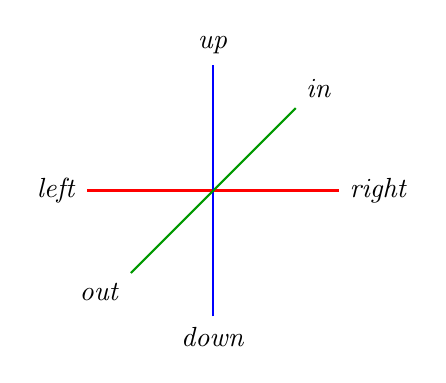
\begin{tikzpicture}[scale=.8]
\draw[thick,red] (-2,0,0) node [black,left] {\textit{left}} -- (2,0,0) node [black,right] {\textit{right}};
\draw[thick,blue] (0,-2,0) node [black,below] {\textit{down}} -- (0,2,0) node [black,above] {\textit{up}};
\draw[thick,green!60!black] (0,0,-3.4) node [black,above right] {\textit{in}} -- (0,0,3.4) node [black,below left] {\textit{out}};
\end{tikzpicture}
\caption{Estrutura de coordenadas tridimensionais}\label{fig.frame}
\end{center}
\end{figure}

Gire o quadro de coordenadas no sentido anti-horário em torno do eixo $z$, de modo que o eixo $z$ permaneça inalterado (Figs.~\ref{fig.standard-axis1}--\ref{fig.rotatez}). A nova orientação do quadro é (\textit{up}, \textit{left}, \textit{out}). Considere agora uma rotação de $90^\circ$ em torno do eixo $x$ (Figs.~ref{fig.standard2}--ref{fig.rotatex}). Isto faz com que o eixo de $y$ salte para fora do papel e o eixo de $z$ caia para baixo sobre o papel, resultando na orientação (\textit{right}, \textit{out}, \textit{down}). Finalmente, considere uma rotação de $90^\circ$ em torno do eixo $y$ (Figs.~\ref{fig.standard-axis3}--\ref{fig.rotatey}). O eixo de $x$ "cai" no papel e o eixo de $z$ "cai para a direita" no papel. A nova posição da moldura é (\textit{in}, \textit{up}, \textit{right}).

\begin{figure}
\begin{minipage}{.48\textwidth}
\begin{tikzpicture}[scale=1.2]
\draw[thick,red,->] (0,0,0) -- (2,0,0) node [black,right] {$x$};
\draw [thick,blue,->] (0,0,0) -- (0,2,0) node [black,above] {$y$};
\draw [thick,green!60!black,->] (0,0,0) -- (0,0,2) node [black,below left] {$z$};
\draw[->] (.5,0,1) arc [start angle=0, end angle=270, radius=3.5mm];
\end{tikzpicture}
\caption{$x$-$y$-$z$ estrutura coordenada}\label{fig.standard-axis1}
\end{minipage}
\hspace{\fill}
\begin{minipage}{.48\textwidth}
\begin{tikzpicture}[scale=1.2]
\draw [thick,blue,->] (0,0,0) -- (-2,0,0) node [black,left] {$y$};
\draw [thick,red,->] (0,0,0) -- (0,2,0) node [black,above] {$x$};
\draw [thick,green!60!black,->] (0,0,0) -- (0,0,2) node [black,below left] {$z$};
\end{tikzpicture}
\caption{$x$-$y$-$z$ quadro coordenado depois de girar $90^\circ$ em torno do eixo $z$}\label{fig.rotatez}
\end{minipage}
\end{figure}


\begin{figure}
\begin{minipage}{.48\textwidth}
\begin{tikzpicture}[scale=1.2]
\draw [thick,red,->] (0,0,0) -- (2,0,0) node [black,right] {$x$};
\draw [thick,blue,->] (0,0,0) -- (0,2,0) node [black,above] {$y$};
\draw [thick,green!60!black,->] (0,0,0) -- (0,0,2) node [black,below left] {$z$};
\draw[->] (1,.1,0) arc [start angle=0, end angle=270, radius=3.5mm];
\end{tikzpicture}
\caption{estrutura coordenada $x$-$y$-$z$}\label{fig.standard-axis2}
\end{minipage}
\hspace{\fill}
\begin{minipage}{.48\textwidth}
\begin{tikzpicture}[baseline=-4em,scale=1.2]
\draw [thick,red,->] (0,0,0) -- (2,0,0) node [black,right] {$x$};
\draw [thick,green!60!black,->] (0,0,0) -- (0,-2,0) node [black,below] {$z$};
\draw [thick,blue,->] (0,0,0) -- (0,0,2) node [black,below left] {$y$};
\end{tikzpicture}
\caption{quadro coordenado depois de girar $90^\circ$ em torno do eixo $x$}\label{fig.rotatex}
\end{minipage}
\end{figure}

\begin{figure}
\begin{minipage}{.48\textwidth}
\begin{tikzpicture}[scale=1.2]
\draw [thick,red,->] (0,0,0) -- (2,0,0) node [black,right] {$x$};
\draw [thick,blue,->] (0,0,0) -- (0,2,0) node [black,above] {$y$};
\draw [thick,green!60!black,->] (0,0,0) -- (0,0,2) node [black,below left] {$z$};
\draw[->] (.3,.8,0) arc [start angle=45, end angle=315, radius=3.5mm];
\end{tikzpicture}
\caption{estrutura coordenada $x$-$y$-$z$}\label{fig.standard-axis3}
\end{minipage}
\hspace{\fill}
\begin{minipage}{.48\textwidth}
\begin{tikzpicture}[baseline=-3.8em,scale=1.2]
\draw [thick,green!60!black,->] (0,0,0) -- (2,0,0) node [black,right] {$z$};
\draw [thick,blue,->] (0,0,0) -- (0,2,0) node [black,above] {$y$};
\draw [thick,red,->] (0,0,0) -- (0,0,-2) node [black,above right] {$x$};
\end{tikzpicture}
\caption{moldura com coordenadas $x$-$y$-$z$ depois de uma rotação de $90^\circ$ em torno do eixo $y$}\label{fig.rotatey}
\end{minipage}
\end{figure}


%\begin{figure}
%\subfigures
%\begin{minipage}{\textwidth}
%\leftfigure{
%\begin{tikzpicture}[scale=1.3]
%\draw[thick,red,->] (0,0,0) -- (2,0,0) node [black,right] {$x$};
%\draw [thick,blue,->] (0,0,0) -- (0,2,0) node [black,above] {$y$};
%\draw [thick,green!60!black,->] (0,0,0) -- (0,0,2) node [black,below left] {$z$};
%\draw[->] (.5,0,1) arc [start angle=0, end angle=270, radius=3.5mm];
%\end{tikzpicture}
%}
%\hspace{\fill}
%\rightfigure{
%\begin{tikzpicture}[scale=1.3]
%\draw [thick,blue,->] (0,0,0) -- (-2,0,0) node [black,left] {$y$};
%\draw [thick,red,->] (0,0,0) -- (0,2,0) node [black,above] {$x$};
%\draw [thick,green!60!black,->] (0,0,0) -- (0,0,2) node [black,below left] {$z$};
%\end{tikzpicture}
%}
%\leftcaption{$x$-$y$-$z$ coordinate frame}\label{fig.standard-axis1}
%\rightcaption{$x$-$y$-$z$ coordinate frame after rotating $90^\circ$ around the $z$-axis}\label{fig.rotatez}
%\end{minipage}
%\end{figure}
%
%
%\begin{figure}
%\subfigures
%\begin{minipage}{\textwidth}
%\leftfigure{
%\begin{tikzpicture}[scale=1.3]
%\draw [thick,red,->] (0,0,0) -- (2,0,0) node [black,right] {$x$};
%\draw [thick,blue,->] (0,0,0) -- (0,2,0) node [black,above] {$y$};
%\draw [thick,green!60!black,->] (0,0,0) -- (0,0,2) node [black,below left] {$z$};
%\draw[->] (1,.1,0) arc [start angle=0, end angle=270, radius=3.5mm];
%\end{tikzpicture}
%}
%\hspace{\fill}
%\rightfigure{
%\begin{tikzpicture}[baseline=-4em,scale=1.3]
%\draw [thick,red,->] (0,0,0) -- (2,0,0) node [black,right] {$x$};
%\draw [thick,green!60!black,->] (0,0,0) -- (0,-2,0) node [black,below] {$z$};
%\draw [thick,blue,->] (0,0,0) -- (0,0,2) node [black,below left] {$y$};
%\end{tikzpicture}
%}
%\leftcaption{$x$-$y$-$z$ coordinate frame}\label{fig.standard-axis2}
%\rightcaption{$x$-$y$-$z$ coordinate frame after rotating $90^\circ$ around the $x$-axis}\label{fig.rotatex}
%\end{minipage}
%\end{figure}
%
%\begin{figure}
%\subfigures
%\begin{minipage}{\textwidth}
%\leftfigure{
%\begin{tikzpicture}[scale=1.3]
%\draw [thick,red,->] (0,0,0) -- (2,0,0) node [black,right] {$x$};
%\draw [thick,blue,->] (0,0,0) -- (0,2,0) node [black,above] {$y$};
%\draw [thick,green!60!black,->] (0,0,0) -- (0,0,2) node [black,below left] {$z$};
%\draw[->] (.3,.8,0) arc [start angle=45, end angle=315, radius=3.5mm];
%\end{tikzpicture}
%}
%\hspace{\fill}
%\rightfigure{
%\begin{tikzpicture}[baseline=-3.8em,scale=1.3]
%\draw [thick,green!60!black,->] (0,0,0) -- (2,0,0) node [black,right] {$z$};
%\draw [thick,blue,->] (0,0,0) -- (0,2,0) node [black,above] {$y$};
%\draw [thick,red,->] (0,0,0) -- (0,0,-2) node [black,above right] {$x$};
%\end{tikzpicture}
%}
%\leftcaption{$x$-$y$-$z$ coordinate frame}\label{fig.standard-axis3}
%\rightcaption{$x$-$y$-$z$ coordinate frame after rotating $90^\circ$ around the $y$-axis}\label{fig.rotatey}
%\end{minipage}
%\end{figure}

\subsection{A regra da direita}

Há duas orientações para cada eixo, $2^3=8$ orientações em geral. O que importa é a orientação relativa de um eixo em relação aos outros dois; por exemplo, uma vez que os eixos $x$- e $y$-eixos foram escolhidos para ficar no plano do papel, o $z$-eixo pode ter sua direção positiva apontando para fora do papel ou para dentro do papel. A escolha deve ser consistente. A convenção em física e mecânica é a regra \emph{direito-mão}. Enrole os dedos de sua mão direita para que eles passem de um eixo para outro eixo. Seu polegar agora aponta para a direção positiva do terceiro eixo. Para os familiares eixos $x$- e $y$- sobre papel, enrole seus dedos no caminho do eixo $x$- para o eixo $y$-. Quando o fizer, seu polegar aponta para fora do papel e isto é tomado como a direção positiva do eixo $z$-eixo. Fig.~\ref{fig.right-hand-rule} mostra o sistema de coordenadas da direita exibido com cada um dos três eixos apontando para fora do papel. De acordo com a regra da direita, as três rotações são:
\begin{quote}
\normalsize
Girar \emph{de} x \emph{para} y por volta de z,\\
Girar \emph{de} y \emph{para} z por volta de x,\\
Girar \emph{de} z \emph{para} x por volta de y.
\end{quote}

\begin{figure}
\begin{center}
\begin{tikzpicture}[scale=.85]
\draw [thick,red,->] (0,0,0) -- (2,0,0) node [black,right] {$x$};
\draw [thick,blue,->] (0,0,0) -- (0,2,0) node [black,above] {$y$};
\draw [thick,green!60!black,->] (0,0,0) -- (0,0,2) node [black,below left] {$z$};
\draw[->] (.5,0,1) arc [start angle=0, end angle=270, radius=3.5mm];
\end{tikzpicture}
\hspace{2em}
\begin{tikzpicture}[scale=.85]
\draw [thick,blue,->] (0,0,0) -- (2,0,0) node [black,right] {$y$};
\draw [thick,green!60!black,->] (0,0,0) -- (0,2,0) node [black,above] {$z$};
\draw [thick,red,->] (0,0,0) -- (0,0,2) node [black,below left] {$x$};
\draw[->] (.5,0,1) arc [start angle=0, end angle=270, radius=3.5mm];
\end{tikzpicture}
\hspace{2em}
\begin{tikzpicture}[scale=.85]
\draw [thick,green!60!black,->] (0,0,0) -- (2,0,0) node [black,right] {$z$};
\draw [thick,red,->] (0,0,0) -- (0,2,0) node [black,above] {$x$};
\draw [thick,blue,->] (0,0,0) -- (0,0,2) node [black,below left] {$y$};
\draw[->] (.5,0,1) arc [start angle=0, end angle=270, radius=3.5mm];
\end{tikzpicture}
\caption{A regra da mão direita}\label{fig.right-hand-rule}
\end{center}
\end{figure}

\subsection{Matrizes para rotações tridimensionais}

Uma matriz de rotação tridimensional é uma matriz de $3\times 3$ porque cada ponto $p$ em uma moldura tem três coordenadas $p_x,p_y,p_z$ que devem ser movidas. 
Comece com uma rotação de $psi$ em torno do eixo $z$, seguida por uma rotação de $theta$ em torno do eixo $y$ e finalmente uma rotação de $phi$ em torno do eixo $x$. Para a primeira rotação em torno do eixo $z$, as coordenadas $x$ e $y$ são giradas como em duas dimensões e a coordenada $z$ permanece inalterada. Portanto, a matriz é:
\[
\spacearray
R_{z(\psi)}=\left[\begin{array}{ccc}\cos\psi&-\sin\psi&0\\\sin\psi&\cos\psi&0\\0&0&1\end{array}\right]\,.
\]
Para a rotação de $\theta$ em torno do eixo $y$, a coordenada $y$ não é alterada e as coordenadas $z$ e $x$ são transformadas ``como se'' fossem as coordenadas $x$ e $y$ de uma rotação em torno do eixo $z$:
\[
\spacearray
R_{y(\theta)}=\left[\begin{array}{ccc}\cos\theta&0&\sin\theta\\0&1&0\\-\sin\theta&0&\cos\theta\\\end{array}\right]\,.
\]
Para a rotação de $\phi$ em torno do eixo $x$, a coordenada $x$ não é alterada e as coordenadas $y$ e $z$ são transformadas ``como se'' fossem as coordenadas $x$ e $y$ de uma rotação em torno do eixo $z$:
\[
\spacearray
R_{x(\phi)}=\left[\begin{array}{ccc}1&0&0\\0&\cos\phi&-\sin\phi\\0&\sin\phi&\cos\phi\\\end{array}\right]\,.
\]
Pode parecer estranho que na matriz para a rotação em torno do eixo $y$ os sinais da função seno tenham mudado. Para convencer-se de que a matriz para esta rotação está correta, redesenhar o diagrama em Fig.~\ref{fig.framea}, substituindo $z$ por $x$ e $x$ por $y$ e realizar o cálculo trigonométrico.

\subsection{Múltiplas rotações}

Há um aviso para compor rotações: como a multiplicação matricial, as rotações tridimensionais \emph{não} comutam. Vamos demonstrar isto através de uma seqüência simples de duas rotações. Considere uma rotação de $90^\circ$ em torno do eixo $z$, seguida por uma rotação de $90^\circ$ em torno do (nova posição do) eixo $x$ (Fig.~\ref{fig.non-commutative1}). O resultado pode ser expresso como (\textit{up}, \textit{out}, \textit{right}).

\begin{figure}
\begin{center}
\begin{tikzpicture}[scale=.85]
\draw [thick,red,->] (0,0,0) -- (2,0,0) node [black,right] {$x$};
\draw [thick,blue,->] (0,0,0) -- (0,2,0) node [black,above] {$y$};
\draw [thick,green!60!black,->] (0,0,0) -- (0,0,2) node [black,below left] {$z$};
\draw[->] (.5,0,1) arc [start angle=0, end angle=270, radius=3.5mm];
\end{tikzpicture}
\hspace{2em}
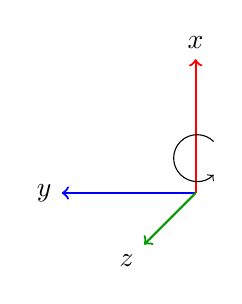
\begin{tikzpicture}[scale=.85]
\draw [thick,blue,->] (0,0,0) -- (-2,0,0) node [black,left] {$y$};
\draw [thick,red,->] (0,0,0) -- (0,2,0) node [black,above] {$x$};
\draw [thick,green!60!black,->] (0,0,0) -- (0,0,2) node [black,below left] {$z$};
\draw[->] (.5,1,.6) arc [start angle=45, end angle=315, radius=3.5mm];
\end{tikzpicture}
\hspace{2em}
\begin{tikzpicture}[scale=.85]
\draw [thick,green!60!black,->] (0,0,0) -- (2,0,0) node [black,right] {$z$};
\draw [thick,red,->] (0,0,0) -- (0,2,0) node [black,above] {$x$};
\draw [thick,blue,->] (0,0,0) -- (0,0,2) node [black,below left] {$y$};
\end{tikzpicture}
\caption{Rotação em torno do eixo de $z$ seguido de rotação em torno do eixo de $x$}\label{fig.non-commutative1}
\end{center}
\end{figure}

Agora considere a operação comutada: uma rotação de $90^\circ$ em torno do eixo $x$, seguida por uma rotação de $90^\circ$ em torno do eixo $z$ (Fig.~\ref{fig.non-commutative2}). O resultado pode ser expresso como (\textit{out}, \textit{left}, \textit{down}), o que não é o mesmo que a orientação anterior.

\begin{figure}
\begin{center}
\begin{tikzpicture}[scale=.85]
\draw [thick,red,->] (0,0,0) -- (2,0,0) node [black,right] {$x$};
\draw [thick,blue,->] (0,0,0) -- (0,2,0) node [black,above] {$y$};
\draw [thick,green!60!black,->] (0,0,0) -- (0,0,2) node [black,below left] {$z$};
\draw[->] (1.4,.1,0) arc [start angle=0, end angle=270, radius=3.5mm];
\end{tikzpicture}
\hspace{2em}
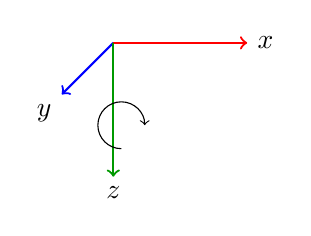
\begin{tikzpicture}[scale=.85,baseline=-3.1em]
\draw [thick,red,->] (0,0,0) -- (2,0,0) node [black,right] {$x$};
\draw [thick,blue,->] (0,0,0) -- (0,0,2) node [black,below left] {$y$};
\draw [thick,green!60!black,->] (0,0,0) -- (0,-2,0) node [black,below] {$z$};
\draw[<-] (.7,-1,.6) arc [start angle=0, end angle=270, radius=3.5mm];
\end{tikzpicture}
\hspace{2em}
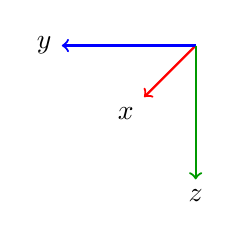
\begin{tikzpicture}[scale=.85,baseline=-3em]
\draw [thick,red,->] (0,0,0) -- (0,0,2) node [black,below left] {$x$};
\draw [thick,blue,->] (0,0,0) -- (-2,0,0) node [black,left] {$y$};
\draw [thick,green!60!black,->] (0,0,0) -- (0,-2,0) node [black,below] {$z$};
\end{tikzpicture}
\caption{Rotação em torno do eixo de $x$ seguido de rotação em torno do eixo de $z$}\label{fig.non-commutative2}
\end{center}
\end{figure}

\subsection{Ângulos de Euler}

Uma rotação arbitrária pode ser obtida por três rotações individuais ao redor dos três eixos, de modo que a matriz para uma rotação arbitrária pode ser obtida multiplicando as matrizes para cada rotação individual. Os ângulos das rotações são chamados \emph{Euler angles}. As fórmulas são um tanto complexas e podem ser encontradas nas referências listadas no final do capítulo. Aqui demonstramos os ângulos de Euler com um exemplo.

\noindent\textbf{Exemplo} A figura~\ref{fig.euler} mostra um quadro de coordenadas girado seqüencialmente $90^\circ$ em torno do eixo $z$, depois o eixo $y$- e finalmente o eixo $x$-. Isto é chamado de rotação do ângulo $zyx$ Euler. A orientação final é (\textit{in}, \textit{up}, \textit{right}).

\begin{figure}
\begin{center}
\begin{tikzpicture}[scale=.7]
\draw [thick,red,->] (0,0,0) -- (2,0,0) node [black,right] {$x$};
\draw [thick,blue,->] (0,0,0) -- (0,2,0) node [black,above] {$y$};
\draw [thick,green!60!black,->] (0,0,0) -- (0,0,2) node [black,below left] {$z$};
\draw[->] (0,-.3,.1) arc [start angle=0, end angle=270, radius=3mm];
\end{tikzpicture}
\hspace{2em}
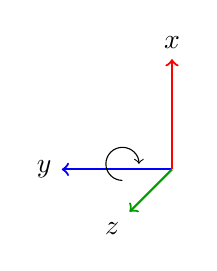
\begin{tikzpicture}[scale=.7]
\draw [thick,blue,->] (0,0,0) -- (-2,0,0) node [black,left] {$y$};
\draw [thick,red,->] (0,0,0) -- (0,2,0) node [black,above] {$x$};
\draw [thick,green!60!black,->] (0,0,0) -- (0,0,2) node [black,below left] {$z$};
\draw[<-] (-.6,.1,0) arc [start angle=0, end angle=270, radius=3mm];
\end{tikzpicture}
\hspace{2em}
\begin{tikzpicture}[scale=.7,baseline=-3em]
\draw [thick,green!60!black,->] (0,0,0) -- (0,2,0) node [black,above] {$z$};
\draw [thick,blue,->] (0,0,0) -- (-2,0,0) node [black,left] {$y$};
\draw [thick,red,->] (0,0,0) -- (0,0,-2.5) node [black,above right] {$x$};
\draw[<-] (.6,.2,-.5) arc [start angle=0, end angle=270, radius=3mm];
\end{tikzpicture}
\hspace{2em}
\begin{tikzpicture}[scale=.7,baseline=-3em]
\draw [thick,blue,->] (0,0,0) -- (0,2,0) node [black,above] {$y$};
\draw [thick,green!60!black,->] (0,0,0) -- (2,0,0) node [black,right] {$z$};
\draw [thick,red,->] (0,0,0) -- (0,0,-2.5) node [black,above right] {$x$};
\end{tikzpicture}
\caption{Ângulos de Euler $zyx$ de $(90^\circ,90^\circ,90^\circ)$}\label{fig.euler}
\end{center}
\end{figure}

Consideremos um manipulador robótico que consiste em uma única junta que pode girar ao redor dos três eixos. Uma seqüência de rotações é realizada como mostrado na Fig.~\ref{fig.euler}. Considere o ponto nas coordenadas $(1,1,1)$ em relação à junta (Fig.~\ref{fig.rotate3}). Após as rotações, quais são as coordenadas deste ponto na moldura fixa original?

\begin{figure}
\begin{minipage}{.48\textwidth}
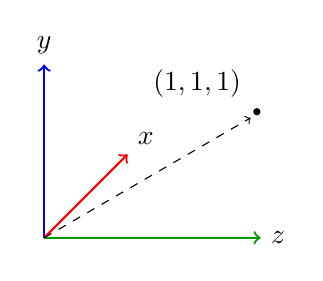
\begin{tikzpicture}[scale=1.1]
\draw [thick,blue,->] (0,0,0) -- (0,2,0) node [black,above] {$y$};
\draw [thick,green!60!black,->] (0,0,0) -- (2.5,0,0) node [black,right] {$z$};
\draw [thick,red,->] (0,0,0) -- (0,0,-2.5) node [black,above right] {$x$};
\draw[->,dashed] (0,0,0) -- (2,1,-1) node[above left,yshift=4pt] {$(1,1,1)$};
\draw[fill] (2,1,-1) circle [xshift=2pt,yshift=2pt,radius=1pt];
\end{tikzpicture}
\caption{Vetor após a rotação final}\label{fig.rotate3}
\end{minipage}
\hspace{\fill}
\begin{minipage}{.48\textwidth}
\begin{tikzpicture}[scale=1.1]
\draw [thick,green!60!black,->] (0,0,0) -- (0,2,0) node [black,above] {$z$};
\draw [thick,blue,->] (0,0,0) -- (-2,0,0) node [black,left] {$y$};
\draw [thick,red,->] (0,0,0) -- (0,0,-2.5) node [black,above right] {$x$};
\draw[<-] (.5,.2,-.8) arc [start angle=0, end angle=270, radius=3mm];
\draw[->,dashed] (0,0,0) -- (2,1,-1) node[above left,yshift=4pt] {$(1,-1,1)$};
\draw[fill] (2,1,-1) circle [xshift=2pt,yshift=2pt,radius=1pt];
\end{tikzpicture}
\caption{Vetor antes de girar em torno do eixo $x$}\label{fig.rotate2}
\end{minipage}
\end{figure}

%\begin{figure}
%\subfigures
%\begin{minipage}{\textwidth}
%\leftfigure{
%\begin{tikzpicture}[scale=1.1]
%\draw [thick,blue,->] (0,0,0) -- (0,2,0) node [black,above] {$y$};
%\draw [thick,green!60!black,->] (0,0,0) -- (2.5,0,0) node [black,right] {$z$};
%\draw [thick,red,->] (0,0,0) -- (0,0,-2.5) node [black,above right] {$x$};
%\draw[->,dashed] (0,0,0) -- (2,1,-1) node[above left,yshift=4pt] {$(1,1,1)$};
%\draw[fill] (2,1,-1) circle [xshift=2pt,yshift=2pt,radius=1pt];
%\end{tikzpicture}
%}
%\hspace{\fill}
%\rightfigure{
%\begin{tikzpicture}[scale=1.1]
%\draw [thick,green!60!black,->] (0,0,0) -- (0,2,0) node [black,above] {$z$};
%\draw [thick,blue,->] (0,0,0) -- (-2,0,0) node [black,left] {$y$};
%\draw [thick,red,->] (0,0,0) -- (0,0,-2.5) node [black,above right] {$x$};
%\draw[<-] (.5,.2,-.8) arc [start angle=0, end angle=270, radius=3mm];
%\draw[->,dashed] (0,0,0) -- (2,1,-1) node[above left,yshift=4pt] {$(1,-1,1)$};
%\draw[fill] (2,1,-1) circle [xshift=2pt,yshift=2pt,radius=1pt];
%\end{tikzpicture}
%}
%\leftcaption{Vector after final rotation}\label{fig.rotate3}
%\rightcaption{Vector before rotating around the $x$-axis}\label{fig.rotate2}
%\end{minipage}
%\end{figure}

Isto pode ser calculado deixando o vetor fixo e considerando as rotações dos quadros de coordenadas. Para alcançar a posição final mostrada na Fig.~\ref{fig.rotate3}, o quadro foi girado em torno do eixo $x$ da orientação mostrada na Fig.~\ref{fig.rotate2}. Examinando a figura, vemos que as coordenadas neste quadro são $(1,-1,1)$. Prosseguindo através dos dois quadros anteriores (Figs.~\ref{fig.rotate1}, \ref{fig.rotate0}), as coordenadas são $(1,-1,-1)$ e $(1,1,-1)$.

\begin{figure}
\begin{minipage}{.48\textwidth}
\begin{tikzpicture}[scale=1.1]
\draw [thick,blue,->] (0,0,0) -- (-2,0,0) node [black,left] {$y$};
\draw [thick,red,->] (0,0,0) -- (0,2,0) node [black,above] {$x$};
\draw [thick,green!60!black,->] (0,0,0) -- (0,0,2) node [black,below left] {$z$};
\draw[<-] (-.6,.1,0) arc [start angle=0, end angle=270, radius=3mm];
\draw[->,dashed] (0,0,0) -- (2,1,-1) node[above left,yshift=4pt] {$(1,-1,-1)$};
\draw[fill] (2,1,-1) circle [xshift=2pt,yshift=2pt,radius=1pt];
\end{tikzpicture}
\caption{Vetor antes da rotação sobre o eixo $y$}\label{fig.rotate1}
\end{minipage}
\hspace{\fill}
\begin{minipage}{.48\textwidth}
\begin{tikzpicture}[scale=1.1]
\draw [thick,red,->] (0,0,0) -- (2.5,0,0) node [black,right] {$x$};
\draw [thick,blue,->] (0,0,0) -- (0,2,0) node [black,above] {$y$};
\draw [thick,green!60!black,->] (0,0,0) -- (0,0,2) node [black,below left] {$z$};
\draw[->] (0,-.3,.1) arc [start angle=0, end angle=270, radius=3mm];
\draw[->,dashed] (0,0,0) -- (2,1,-1) node[above left,yshift=4pt] {$(1,1,-1)$};
\draw[fill] (2,1,-1) circle [xshift=2pt,yshift=2pt,radius=1pt];
\end{tikzpicture}
\caption{Vetor no quadro fixo antes de girar em torno do eixo de $z$}.
\label{fig.rotate0}
\end{minipage}
\end{figure}

%\begin{figure}
%\subfigures
%\begin{minipage}{\textwidth}
%\leftfigure{
%\begin{tikzpicture}[scale=1.1]
%\draw [thick,blue,->] (0,0,0) -- (-2,0,0) node [black,left] {$y$};
%\draw [thick,red,->] (0,0,0) -- (0,2,0) node [black,above] {$x$};
%\draw [thick,green!60!black,->] (0,0,0) -- (0,0,2) node [black,below left] {$z$};
%\draw[<-] (-.6,.1,0) arc [start angle=0, end angle=270, radius=3mm];
%\draw[->,dashed] (0,0,0) -- (2,1,-1) node[above left,yshift=4pt] {$(1,-1,-1)$};
%\draw[fill] (2,1,-1) circle [xshift=2pt,yshift=2pt,radius=1pt];
%\end{tikzpicture}
%}
%\hspace{\fill}
%\rightfigure{
%\begin{tikzpicture}[scale=1.1]
%\draw [thick,red,->] (0,0,0) -- (2.5,0,0) node [black,right] {$x$};
%\draw [thick,blue,->] (0,0,0) -- (0,2,0) node [black,above] {$y$};
%\draw [thick,green!60!black,->] (0,0,0) -- (0,0,2) node [black,below left] {$z$};
%\draw[->] (0,-.3,.1) arc [start angle=0, end angle=270, radius=3mm];
%\draw[->,dashed] (0,0,0) -- (2,1,-1) node[above left,yshift=4pt] {$(1,1,-1)$};
%\draw[fill] (2,1,-1) circle [xshift=2pt,yshift=2pt,radius=1pt];
%\end{tikzpicture}
%}
%\leftcaption{Vector before rotating around the $y$-axis}\label{fig.rotate1}
%\rightcaption{Vector in the fixed frame before rotating around the $z$-axis}\label{fig.rotate0}
%\end{minipage}
%\end{figure}

Estas coordenadas podem ser calculadas a partir das matrizes de rotação para as rotações em torno dos três eixos. As coordenadas do quadro de coordenadas final são $(1,1,1)$, portanto, no quadro antes da rotação em torno do eixo $x$- as coordenadas eram:
\[
\spacearray
\left[\begin{array}{ccc}1&0&0\\0&0&-1\\0&1&0\\\end{array}\right]
\left[\begin{array}{c}1\\1\\1\end{array}\right]=
\left[\begin{array}{c}1\\-1\\1\end{array}\right]\,.
\]
As coordenadas no quadro antes da rotação em torno do eixo $y$-ei:
\[
\spacearray
\left[\begin{array}{ccc}0&0&1\\0&1&0\\-1&0&0\\\end{array}\right]
\left[\begin{array}{c}1\\-1\\1\end{array}\right]=
\left[\begin{array}{c}1\\-1\\-1\end{array}\right]\,.
\]
Finalmente, as coordenadas no quadro fixo antes da rotação em torno do eixo de $z$ foram:
\[
\spacearray
\left[\begin{array}{ccc}0&-1&0\\1&0&0\\0&0&1\\\end{array}\right]
\left[\begin{array}{c}1\\-1\\-1\end{array}\right]=
\left[\begin{array}{c}1\\1\\-1\end{array}\right]\,.
\]
Para três rotações arbitrárias do ângulo $zyx$ Euler: $\psi$ em torno do eixo $z$, depois $\theta$ em torno do eixo $y$ e finalmente $\phi$ em torno do eixo $x$, a matriz de rotação é:
\[
R=R_{z(\psi)}R_{y(\theta)}R_{x(\phi)}\,.
\]
Pode parecer estranho que a ordem da multiplicação da matriz (que é sempre da direita para a esquerda) seja oposta à ordem das rotações. Isto porque estamos tomando um vetor no quadro de coordenadas final e transformando-o de volta no quadro fixo para determinar suas coordenadas no quadro fixo.

\begin{framed}
\act{Ângulos múltiplos de Euler}{euler-multiple}
\begin{itemize}
\item Multiplique as três matrizes para obter uma única matriz que transforme diretamente as coordenadas de $(1,1,1)$ para $(1,1,-1)$.
\item Faça o mesmo cálculo para outras rotações, alterando a seqüência dos eixos e os ângulos de rotação.
\end{itemize}
\end{framed}

\subsection{O número de rotações de ângulo Euler distintas}

Há três eixos, portanto deve haver $3^3=27$ seqüências de ângulos de Euler. Entretanto, não faz sentido girar duas vezes sucessivamente em torno do mesmo eixo porque o mesmo resultado pode ser obtido girando uma vez pela soma dos ângulos, de modo que há apenas $3\cdot 2\cdot 2=12$ diferentes seqüências de ângulos de Euler.  A seguinte atividade pede que você explore diferentes seqüências de ângulos de Euler.

\begin{framed}
\act{Distintos ângulos de Euler}{euler-distinct}
\begin{itemize}
\item Para experimentar as rotações tridimensionais, é útil construir uma moldura coordenada a partir de três lápis ou palhetas mutuamente perpendiculares.
\item Desenhar as armações de coordenadas para uma rotação angular de $zyz$ Euler, onde cada rotação é por $90^\circ$. %Answer: $(l,o,u)$
\item A rotação de $zyz$ dá o mesmo resultado na rotação de $zyx$ mostrada em Fig.~\ref{fig.euler}? %Answer: $(0,90,0)$
\item Experiência com outras seqüências de rotação e com outros ângulos que não $90^\circ$.
\end{itemize}
\end{framed}

\section{Advanced topics in three-dimensional transforms}\label{s.advanced-three}

Agora que você já provou as rotações tridimensionais, pesquisamos os próximos passos no aprendizado deste tópico que você pode estudar nos livros didáticos listados nas referências.

Existem ângulos de Euler de $12$ e a escolha dos quais utilizar depende da aplicação pretendida. Além disso, há uma maneira diferente de definir as rotações. Os ângulos de Euler são \emph{eixos móveis} transformadas, isto é, cada um dos eixos  cada rotação está em torno da posição \emph{new} do eixo após a rotação anterior. Na Fig.~\ref{fig.euler}, a segunda rotação está em torno do eixo $y$- que agora aponta para a esquerda, não em torno do eixo $y$- original que aponta para cima. Também é possível definir as rotações \emph{eixos fixos} nas quais as rotações subseqüentes estão em torno dos eixos originais do sistema de coordenadas. Em três dimensões, as transformações homogêneas que incluem traduções além das rotações podem ser representadas de forma eficiente como matrizes de $4\times 4$.

Os ângulos de Euler são relativamente ineficientes para calcular e sofrem com as instabilidades computacionais. Estas podem ser superadas usando \emph{quaternions}, que são uma generalização de números complexos. Os Quaternions utilizam três números ``imaginários'', $i,j,k$, onde:
\[
i^2 = j^2 = k^2 = ij\,k = -1\,.
\]
Lembre-se de que um vetor no plano bidimensional pode ser expresso como um número complexo $x+\vec{i},y$. A rotação do vetor por um ângulo $\theta$ pode ser realizada multiplicando pelo valor $\cos \theta + \vec{i} \sin\theta$.  Da mesma forma, em três dimensões, um vetor pode ser expresso como um quaternion com um componente real zero:$p=0+x\,\vec{i} + y\,\vec{j} + z\,\vec{k}$. Dado um eixo e um ângulo, existe um quaternion $q$ que gira o vetor em torno do eixo por este ângulo usando a fórmula $qpq^{-1}$. Este cálculo é mais eficiente e robusto do que o cálculo equivalente com ângulos Euler e é usado em uma variedade de contextos, como controle de aeronaves e computação gráfica.


\section{Sumário}

A cinemática é a descrição do movimento de um robô. Na cinemática dianteira, recebemos um conjunto de comandos para o robô e precisamos computar sua posição final em relação à posição inicial. Na cinemática inversa, nos é dada uma posição final desejada e precisamos computar os comandos que levarão o robô a essa posição. Este capítulo demonstrou cálculos cinemáticos para um braço manipulador robótico bidimensional simples. Na prática, os manipuladores se movimentam em três dimensões e os cálculos são mais difíceis. Soluções exatas para computação da cinemática inversa geralmente não podem ser encontradas e são usadas soluções numéricas aproximadas.

Há muitas maneiras de definir e computar rotações arbitrárias. Mencionamos os ângulos de Euler onde uma rotação arbitrária é obtida por uma seqüência de três rotações em torno dos eixos coordenados. Quaternions, uma generalização de números complexos, são freqüentemente utilizados na prática porque são computacionalmente mais eficientes e robustos.

\section{Outras leituras}

Os livros didáticos avançados sobre cinemática robótica e tópicos relacionados são os de Craig \cite{craig} e Spong et al. \cite{spong}. Veja também o Capítulo 3 do Correll \cite{correll}. O Apêndice B de \cite{craig} contém as matrizes de rotação para todas as seqüências de ângulos de Euler. As vídeo-palestras de Angela Sodemann são muito úteis:\\
\url{https://www.youtube.com/user/asodemann3},\\
\url{http://www.robogrok.com/Flowchart.html}.

Embora não seja um livro sobre robótica, a monografia de Vince sobre quaternions \cite{vince} dá uma excelente apresentação da matemática das rotações.
